\chapter[ESPACIOS VECTORIALES REALES]{ESPACIOS VECTORIALES \\ REALES}\label{chap:ev}

En las páginas siguientes, exploraremos los espacios vectoriales, estructuras fundamentales en matemáticas que sustentan numerosos campos científicos y tecnológicos. Un espacio vectorial real se define mediante diez axiomas básicos, algo que debe comprenderse como un conjunto de principios que no se \emph{demuestran}; más bien, son suposiciones que sirven como punto de partida para desarrollar teoremas.

\section{Definición y ejemplos}

\begin{definicion}{}{espvec}
    Sea $V$ un conjunto no vacío y sea $K$ un campo. Definimos la suma de elementos en $V$ y una multiplicación por un escalar respectivamente, como
    \begin{alignat*}{2}
        + &: & \quad V \times V & \longrightarrow V \\
        & & (\mathbb{u}, \mathbb{v}) & \longmapsto \mathbb{u} + \mathbb{v} \\
        & \\
        \cdot &: & \quad K \times V & \longrightarrow V \\
        & & (\alpha, \mathbb{u}) & \longmapsto \alpha \cdot \mathbb{u}
    \end{alignat*}
    Decimos que $V$ es un \emph{espacio vectorial sobre $K$}, si cumple con los siguientes axiomas: Para toda $\mathbb{x}$, $\mathbb{y}$, $\mathbb{z} \in V$ y $\alpha$, $\beta \in K$
    \begin{enumerate}[label=\roman*), topsep=6pt, itemsep=0pt]
        \item Cerradura: $\mathbb{x} + \mathbb{y} \in V$.
        \item Asociatividad: $\mathbb{x} + (\mathbb{y} + \mathbb {z}) = (\mathbb{x} + \mathbb{y}) + \mathbb{z}$.\newpage
        \item Conmutatividad: $\mathbb{x} + \mathbb{y} = \mathbb{y} + \mathbb{x}$.
        \item Neutro aditivo: Existe un elemento $\mathbb{0} \in V$ que llamaremos cero tal que $\mathbb{x} + \mathbb{0} = \mathbb{0} + \mathbb{x} = \mathbb{x}$.
        \item Inverso aditivo: Para cada $\mathbb{x} \in V$, existe un elemento $-\mathbb{x} \in V$ tal que $\mathbb{x} + (-\mathbb{x}) = \mathbb{0}$. A $-\mathbb{x}$ se le llama inverso de $\mathbb{x}$.
        \item Cerradura: $\alpha \cdot \mathbb{x} \in V$.
        \item Asociatividad: $\alpha \cdot (\beta \cdot \mathbb{x}) = (\alpha \cdot \beta) \cdot \mathbb{x}$.
        \item Distributividad (con un escalar): $\alpha \cdot (\mathbb{x} + \mathbb{y}) = \alpha \mathbb{x} + \alpha \mathbb{y}$.
        \item Distributividad (con dos escalares): $(\alpha + \beta) \cdot \mathbb{x} = \alpha \mathbb{x} + \beta \mathbb{x}$.
        \item Identidad multiplicativa: $1 \cdot \mathbb{x} = \mathbb{x}$.
    \end{enumerate}
\end{definicion}

Si $V$ es un espacio vectorial sobre un campo $K$ y $\mathbb{u} \in V$, entonces diremos que $\mathbb{u}$ es un \emph{vector}. A menos que se indique lo contrario, asumiremos que el campo $K$ es $\RR$, es decir, que trabajamos con espacios vectoriales reales.

\begin{theorem}{}{}
    \TituloBox{Unicidad del neutro y el inverso aditivo:} En un espacio vectorial $V$ sobre $K$, el inverso y el neutro aditivo son únicos.

    \tcblower
    \demostracion Veamos primero que el neutro aditivo es único. Del axioma iv), existe $\mathbb{0} \in V$ tal que para toda $\mathbb{x} \in V$
    \begin{equation}
        \mathbb{x} + \mathbb{0} = \mathbb{0} + \mathbb{x} = \mathbb{x} \label{ec1}
    \end{equation}
    Supongamos que existe $\tilde{\mathbb{0}} \in V$ tal que
    \begin{equation}
        \mathbb{x} + \tilde{\mathbb{0}} = \tilde{\mathbb{0}} + \mathbb{x} = \mathbb{x} \label{ec2}
    \end{equation}
    de \eqref{ec1}, como se cumple para toda $\mathbb{x} \in V$, en particular se cumple para $\mathbb{x} = \tilde{\mathbb{0}}$, es decir
    \begin{equation}
        \tilde{\mathbb{0}} + \mathbb{0} = \mathbb{0} + \tilde{\mathbb{0}} = \tilde{\mathbb{0}} \label{ec3}
    \end{equation}
    de igual forma, de la expresión \eqref{ec2} se cumple para toda $\mathbb{x} \in V$, en particular, para $\mathbb{x} = \mathbb{0}$. Así
    \begin{equation}
        \mathbb{0} + \tilde{\mathbb{0}} = \tilde{\mathbb{0}} + \mathbb{0} = \mathbb{0} \label{ec4}
    \end{equation}
    de \eqref{ec4} y \eqref{ec3},
    \begin{equation*}
        \tilde{\mathbb{0}} \stackrel{\eqref{ec3}}{=} \mathbb{0} + \tilde{\mathbb{0}} \stackrel{\eqref{ec4}}{=} \mathbb{0}
    \end{equation*}
    Por tanto, $\tilde{\mathbb{0}} = \mathbb{0}$. Ahora, demostremos que el inverso es único. Del axioma v), tenemos que para cada $\mathbb{x} \in V$ existe $-\mathbb{x}$ tal que
    \begin{equation}
        \mathbb{x} + (-\mathbb{x}) = \mathbb{0} \label{ec5}
    \end{equation}
    Supongamos que existe $\mathbb{y} \in V$ tal que
    \begin{equation}
        \mathbb{x} + \mathbb{y} = \mathbb{0} \label{ec6}
    \end{equation}
    Demostraremos que $\mathbb{y} = -\mathbb{x}$
    \begin{align*}
        \mathbb{y} & = \mathbb{y} + \mathbb{0} && \text{por axioma iv)} \\
        & = \mathbb{y} + \big( \mathbb{x} + (-\mathbb{x}) \big) && \text{por axioma v)} \\
        & = (\mathbb{y} + \mathbb{x}) + (-\mathbb{x}) && \text{por axioma ii)} \\
        & = (\mathbb{x} + \mathbb{y}) + (-\mathbb{x}) && \text{por axioma iii)} \\
        & = \mathbb{0} + (-\mathbb{x}) && \text{por la expresión \eqref{ec6}} \\
        & = -\mathbb{x} && \text{por axioma iv)}
    \end{align*}
    Por lo tanto, $\mathbb{y} = -\mathbb{x}$.
\end{theorem}

\newpage

\begin{theorem}{}{}
    Sea $V$ un espacio vectorial sobre $K$, entonces
    \begin{enumerate}[label=\roman*., topsep=6pt, itemsep=0pt]
        \item $\alpha \cdot \mathbb{0} = \mathbb{0}$, $\forall \alpha \in K$.
        \item $0 \cdot \mathbb{x} = \mathbb{0}$, $\forall \mathbb{x} \in V$.
        \item Si $\alpha \cdot \mathbb{x} = \mathbb{0}$, entonces $\alpha = 0$ o $\mathbb{x} = \mathbb{0}$.
        \item $(-1) \cdot \mathbb{x} = - \mathbb{x}$.
    \end{enumerate}

    \tcblower
    \demostracion
    \begin{enumerate}[label=\roman*., topsep=6pt, itemsep=0pt]
        \item Sea $\alpha \in K$, tenemos que
        \begin{align}
            \mathbb{0} & = \mathbb{0} + \mathbb{0} && \text{por axioma iv)} \label{ec7} \\
            & = \alpha \cdot \mathbb{0} + (-\alpha \cdot \mathbb{0}) && \text{por axioma v)} \label{ec8}
        \end{align}
        de \eqref{ec7},
        \begin{align}
            \alpha \cdot \mathbb{0} & = \alpha \cdot (\mathbb{0} + \mathbb{0}) && \text{por def. de producto escalar} \label{ec9} \\
            & = \alpha \cdot \mathbb{0} + \alpha \cdot \mathbb{0} && \text{por axioma viii)} \label{ec10}
        \end{align}
        sustituyendo \eqref{ec10} en la ecuación \eqref{ec8}, obtenemos
        \begin{align*}
            \mathbb{0} & = (\alpha \cdot \mathbb{0} + \alpha \cdot \mathbb{0}) + (-\alpha \cdot \mathbb{0}) \\
            & = \alpha \cdot \mathbb{0} + \big( \alpha \cdot \mathbb{0} + (-\alpha \cdot \mathbb{0}) \big) && \text{por axioma ii)} \\
            & = \alpha \cdot \mathbb{0} + \mathbb{0} && \text{por axioma v)} \\
            & = \alpha \cdot \mathbb{0} && \text{por axioma iv)}
        \end{align*}
        Por tanto, $\alpha \cdot \mathbb{0} = \mathbb{0}$.
        \item Sea $\mathbb{x} \in V$. Sabemos que en $K = \RR$, se cumple que $0 + 0 = 0$, ahora
        \begin{align}
            0 \cdot \mathbb{x} & = (0 + 0) \cdot \mathbb{x} && \text{por def. de producto escalar} \label{ec11} \\
            & = 0 \cdot \mathbb{x} + 0 \cdot \mathbb{x} && \text{por ix)} \label{ec12}
        \end{align}
        Por otra parte,
        \begin{align}
            \mathbb{0} & = 0 \cdot \mathbb{x} + (-0 \cdot \mathbb{x}) && \text{por axioma v)} \label{ec13}
        \end{align}
        Sustituyendo \eqref{ec12} en \eqref{ec13},
        \begin{align*}
            \mathbb{0} & = (0 \cdot \mathbb{0} + 0 \cdot \mathbb{0}) + (-0 \cdot \mathbb{x}) \\
            & = 0 \cdot 0 + \big( 0 \cdot \mathbb{x} + (-0 \cdot \mathbb{x}) \big) && \text{por axioma ii)} \\
            & = 0 \cdot \mathbb{x} + 0 && \text{por axioma v)} \\
            & = 0 \cdot \mathbb{x} && \text{por axioma iv)}
        \end{align*}
        Por tanto, $0 \cdot \mathbb{x} = \mathbb{0}$.
        \item Supongamos que $\alpha \neq 0$, entonces hay que demostrar que $\mathbb{x} = \mathbb{0}$. Como $\alpha \in K$ y $\alpha \neq 0$, entonces existe $\alpha^{-1} \in K$ tal que
        \begin{equation}
            \alpha^{-1} \cdot \alpha = 1 \label{ec14}
        \end{equation}
        De la hipótesis,
        \begin{align*}
            \mathbb{0} & = \alpha^{-1} \cdot \mathbb{0} && \text{por (i) de este teorema} \\
            & = \alpha^{-1} \cdot (\alpha \cdot \mathbb{x}) && \text{por hipótesis} \\
            & = (\alpha^{-1} \cdot \alpha) \cdot \mathbb{x} && \text{por axioma vii)} \\
            & = 1 \cdot \mathbb{x} && \text{por ecuación \eqref{ec14}} \\
            & = \mathbb{x} && \text{por axioma x)}
        \end{align*}
        Por tanto, $\mathbb{x} = \mathbb{0}$. Ahora, supongamos que $\mathbb{x} = \mathbb{0}$. Procedamos por reducción al absurdo, supongamos que $\alpha \neq 0$, entonces existe $\alpha^{-1} \in K$ tal que
        \begin{equation}
            \alpha^{-1} \cdot \alpha = 1 \label{ec15}
        \end{equation}
        Entonces
        \begin{align*}
            \mathbb{x} & = 1 \cdot \mathbb{x} && \text{por axioma x)} \\
            & = (\alpha^{-1} \cdot \alpha) \cdot \mathbb{x} && \text{por la ecuación \eqref{ec15}} \\
            & = \alpha^{-1} \cdot (\alpha \cdot \mathbb{x}) && \text{por axioma vii)} \\
            & = \alpha^{-1} \cdot \mathbb{0} && \text{por hipótesis} \\
            & = \mathbb{0}
        \end{align*}
        Por lo tanto, $\mathbb{x} = \mathbb{0}$, como se quería demostrar. Ahora, si $\alpha = 0$ y $\mathbb{x} = \mathbb{0}$, la propiedad (iii) queda demostrada por los incisos (i) y (ii) de este teorema.
        \item Como
        \begin{equation}
            0 = 1 + (-1) \in K \label{ec16}
        \end{equation}
        por (i) de este teorema,
        \begin{align*}
            \mathbb{0} & = 0 \cdot \mathbb{x} \\
            & = \big( 1 + (-1) \big) \cdot \mathbb{x} && \text{por la expresión \eqref{ec16}} \\
            & = 1 \cdot \mathbb{x} +  (-1) \cdot \mathbb{x} && \text{por axioma ix)}
        \end{align*}
        esto es
        \begin{equation}
            \mathbb{0} = 1 \cdot \mathbb{x} + (-1) \cdot \mathbb{x} \label{ec17}
        \end{equation}
        Ahora,
        \begin{align*}
            -\mathbb{x} & = - \mathbb{x} + \mathbb{0} \\
            & = -\mathbb{x} + \big( 1 \cdot \mathbb{x} + (-1) \cdot \mathbb{x} \big) && \text{por la expresión \eqref{ec17}} \\
            & = (-\mathbb{x} + 1 \cdot \mathbb{x}) + (-1) \cdot \mathbb{x} && \text{por axioma ii)} \\
            & = (-\mathbb{x} + \mathbb{x}) + (-1) \cdot \mathbb{x} && \text{por axioma x)} \\
            & = \mathbb{0} + (-1) \cdot \mathbb{x} && \text{por axioma v)} \\
            & = (-1) \cdot \mathbb{x} && \text{por axioma iv)}
        \end{align*}
        Por tanto, $-\mathbb{x} = (-1) \cdot \mathbb{x}$.
    \end{enumerate}
\end{theorem}

En el siguiente ejemplo, demostraremos que $\RR[2]$ es un espacio vectorial sobre $\RR$, verificando que cumple con todas las propiedades que definen un espacio vectorial.\sideFigure[\label{JAJAJJAJS}]{\vspace{6cm}
\begin{center}
    \begin{tikzpicture}%[scale=0.83]
        \coordinate (A) at (1,2.5);
        \coordinate (B) at (2.5,1);
        \coordinate (C) at (3.5,3.5);
        \coordinate (D) at ($1.4*(B)$);
        %
        \draw[thick,-Stealth] (-0.5,0) -- (4.5,0);
        \draw[thick,-Stealth] (0,-0.5) -- (0,4.5);
        \draw[dash pattern=on 3pt off 3pt] (A) -- (C) -- (B);
        \draw[dash pattern=on 3pt off 3pt] (0,3.5) node[left] {$b + d$} -- (3.5,3.5) -- (3.5,0) node[below] {$a + c$};
        \draw[dash pattern=on 3pt off 3pt] (0,2.5) node[left] {$d$} -- (1,2.5) -- (1,0) node[below] {$c$};
        \draw[dash pattern=on 3pt off 3pt] (0,1) node[left] {$b$} -- (2.5,1) -- (2.5,0) node[below] {$a$};
        \draw[-latex] (0,0) -- (A);
        \draw[-latex] (0,0) -- (B);
        \draw[-latex] (0,0) -- (C) node [right] {$\begin{pmatrix} a + c \\ b + d \end{pmatrix}$};
        \draw[-latex] (0,0) -- (D) node [right] {$\begin{pmatrix} \alpha a \\ \alpha b \end{pmatrix}$};
    \end{tikzpicture}
\end{center}
}

\begin{examplebox}{}{}
    Recordemos por el curso de Geometría Analítica que
    $$\RR[2] = \left\{ \begin{pmatrix}
        x \\
        y
    \end{pmatrix} \mid x \in \RR, y \in \RR \right\}$$
    en el cual se definen dos operaciones dados $\mathbb{x}$, $\mathbb{y} \in \RR[2]$ con $\mathbb{x} = \begin{pmatrix}
        a \\
        b
    \end{pmatrix}$ e $\mathbb{y} = \begin{pmatrix}
        c \\
        d
    \end{pmatrix}$
    \begin{alignat*}{2}
        + &: & \quad \RR[2] \times \RR[2] & \longrightarrow \RR[2] \\
        & & (\mathbb{x}, \mathbb{y}) & \longmapsto \begin{pmatrix}
            a + c \\
            b + d
        \end{pmatrix} \\
        & \\
        \cdot &: & \quad \RR \times \RR[2] & \longrightarrow \RR[2] \\
        & & (\alpha, \mathbb{x}) & \longmapsto \begin{pmatrix}
            \alpha a \\
            \alpha b
        \end{pmatrix}
    \end{alignat*}
    Notemos que las operaciones antes mencionadas admiten una interpretación geométrica (vea la figura \ref{JAJAJJAJS}). El conjunto $\RR[2]$ representa el conjunto de todos los pares ordenados de números reales. $\RR[2]$ es bidimensional, lo que significa que tiene dos dimensiones: la dimensión horizontal (eje $x$ por convención) y la dimensión vertical (eje $y$ por convención). En geometría analítica, se utiliza para representar figuras geométricas, ecuaciones de rectas, círculos y cualquier otra forma bidimensional. Probemos que $V = \RR[2]$, con las operaciones “$+$” y “$\cdot$” definidas previamente es un espacio vectorial sobre $\RR$. Verifiquemos los diez axiomas de un espacio vectorial (definición \ref{definicion:espvec}) como sigue:
    \begin{enumerate}[label=\roman*), topsep=6pt, itemsep=0pt]
        \item Sea $\mathbb{x}$, $\mathbb{y} \in \RR[2]$ con $\mathbb{x} = \begin{pmatrix}
            a \\
            b
        \end{pmatrix}$, $\displaystyle \mathbb{y} = \begin{pmatrix}
            c \\
            d
        \end{pmatrix}$, entonces
        \begin{align*}
            \mathbb{x} + \mathbb{y} & = \begin{pmatrix}
                a \\
                b
            \end{pmatrix} + \begin{pmatrix}
                c \\
                d
            \end{pmatrix} \\
            & = \begin{pmatrix}
                a + c \\
                b + d
            \end{pmatrix} && \text{por def. de suma} \\
            & = \begin{pmatrix}
                a + c \\
                b + d
            \end{pmatrix} \in \RR[2]
        \end{align*}
        Ya que $a$, $b$, $c$, $d \in \RR$, entonces $a+c$, $b+d \in \RR$. Por tanto, se cumple la propiedad de cerradura.
        \item Sea $\mathbb{x}$, $\mathbb{y}$, $\mathbb{z} \in \RR[2]$ con $\mathbb{x} = \begin{pmatrix}
            a \\
            b
        \end{pmatrix}$, $\mathbb{y} = \begin{pmatrix}
            c \\
            d
        \end{pmatrix}$, $\mathbb{z} = \begin{pmatrix}
            m \\
            l
        \end{pmatrix}$, entonces
        \begin{align*}
            \mathbb{x} + (\mathbb{y} + \mathbb{z}) & = \begin{pmatrix}
                a \\
                b
            \end{pmatrix} + \left[ \begin{pmatrix}
                c \\
                d
            \end{pmatrix} + \begin{pmatrix}
                m \\
                l
            \end{pmatrix} \right] \\
            & = \begin{pmatrix}
                a \\
                b
            \end{pmatrix} + \begin{pmatrix}
                c + m \\
                d + l
            \end{pmatrix} && \text{por def. de suma} \\
            & = \begin{pmatrix}
                a + (c + m) \\
                b + (d + l)
            \end{pmatrix} && \text{por def. de suma} \\
            & = \begin{pmatrix}
                (a + c) + m \\
                (b + d) + l
            \end{pmatrix} && \text{por asociatividad en $\RR$} \\
            & = \begin{pmatrix}
                a + c \\
                b + d
            \end{pmatrix} + \begin{pmatrix}
                m \\
                l
            \end{pmatrix} && \text{por def. de suma} \\
            & = \left[ \begin{pmatrix}
                a \\
                b
            \end{pmatrix} + \begin{pmatrix}
                c \\
                d
            \end{pmatrix} \right] + \begin{pmatrix}
                m \\
                l
            \end{pmatrix} && \text{por def. de suma} \\
            & = (\mathbb{x} + \mathbb{y}) + \mathbb{z}
        \end{align*}
        Por tanto, se cumple la asociatividad.
        \item Sea $\mathbb{x}$, $\mathbb{y} \in \RR[2]$ con $\mathbb{x} = \begin{pmatrix}
            a \\
            b
        \end{pmatrix}$, $\mathbb{y} = \begin{pmatrix}
            c \\
            d
        \end{pmatrix}$, entonces
        \begin{align*}
            \mathbb{x} + \mathbb{y} & = \begin{pmatrix}
                a \\
                b
            \end{pmatrix} + \begin{pmatrix}
                c \\
                d
            \end{pmatrix} \\
            & = \begin{pmatrix}
                a + c \\
                b + d
            \end{pmatrix} && \text{por def. de suma} \\
            & = \begin{pmatrix}
                c + a \\
                d + b
            \end{pmatrix} && \text{por conmutatividad en $\RR$} \\
            & = \begin{pmatrix}
                c \\
                d
            \end{pmatrix} + \begin{pmatrix}
                a \\
                b
            \end{pmatrix} && \text{por def. de suma} \\
            & = \mathbb{y} + \mathbb{x}
        \end{align*}
        Por tanto, se cumple la conmutatividad.
        \item Sea $\mathbb{0} \in \RR[2]$ con $\mathbb{0} = \begin{pmatrix}
            0 \\
            0
        \end{pmatrix}$, entonces
        \begin{align*}
            \mathbb{0} + \mathbb{x} & = \begin{pmatrix}
                0 \\
                0
            \end{pmatrix} + \begin{pmatrix}
                a \\
                b
            \end{pmatrix} \\
            & = \begin{pmatrix}
                0 + a \\
                0 + b
            \end{pmatrix} && \text{por def. de suma} \\
            & = \begin{pmatrix}
                a \\
                b
            \end{pmatrix} && \text{por neutro aditivo en $\RR$} \\
            & = \mathbb{x}
        \end{align*}
        Por tanto, se cumple la propiedad del neutro aditivo.
        \item Dado $\mathbb{x} = \begin{pmatrix}
            a \\
            b
        \end{pmatrix}$, existe $-\mathbb{x} = \begin{pmatrix}
            -a \\
            -b
        \end{pmatrix} \in \RR[2]$ tal que
        \begin{align*}
            \mathbb{x} + (-\mathbb{x}) & = \begin{pmatrix}
                a \\
                b
            \end{pmatrix} + \begin{pmatrix}
                -a \\
                -b
            \end{pmatrix} \\
            & = \begin{pmatrix}
                a + (-a) \\
                b + (-b)
            \end{pmatrix} && \text{por def. de suma} \\
            & = \begin{pmatrix}
                a - a \\
                b - b
            \end{pmatrix} && \text{por definición en $\RR$} \\
            & = \begin{pmatrix}
                0 \\
                0
            \end{pmatrix} && \text{por inv. aditivo en $\RR$} \\
            & = \mathbb{0}
        \end{align*}
        Por tanto, se cumple la propiedad del inverso aditivo.
        \item Sea $\alpha \in \RR$ y sea $\mathbb{x} \in \RR[2]$ con $\mathbb{x} = \begin{pmatrix}
            a \\
            b
        \end{pmatrix}$, entonces
        \begin{align*}
            \alpha \cdot \mathbb{x} & = \alpha \cdot \begin{pmatrix}
                a \\
                b
            \end{pmatrix} \\
            & = \begin{pmatrix}
                \alpha a \\
                \alpha b
            \end{pmatrix} \in \RR[2] && \text{por def. de producto}
        \end{align*}
        Ya que $\alpha a$, $\alpha b \in \RR$, se cumple la propiedad de cerradura.
        \item Sea $\alpha$, $\beta \in \RR$ y sea $\mathbb{x} \in \RR[2]$ con $\mathbb{x} = \begin{pmatrix}
            a \\
            b
        \end{pmatrix}$, entonces
        \begin{align*}
            \alpha \cdot (\beta \cdot \mathbb{x}) & = \alpha \cdot \left[ \beta \cdot \begin{pmatrix}
                a \\
                b
            \end{pmatrix} \right] \\
            & = \alpha \cdot \left[ \begin{pmatrix}
                \beta a \\
                \beta b
            \end{pmatrix} \right] && \text{por def. de producto} \\
            & = \begin{pmatrix}
                \alpha (\beta a) \\
                \alpha (\beta b)
            \end{pmatrix} && \text{por def. de producto} \\
            & = \begin{pmatrix}
                (\alpha \beta) a \\
                (\alpha \beta) b
            \end{pmatrix} && \text{por asociatividad en $\RR$} \\
            & = (\alpha\beta) \cdot \begin{pmatrix}
                a \\
                b
            \end{pmatrix} && \text{por def. de producto} \\
            & = (\alpha\beta) \cdot \mathbb{x}
        \end{align*}
        Por tanto, se cumple la asociatividad.
        \item Sea $\alpha \in \RR$ y sean $\mathbb{x}$, $\mathbb{y} \in \RR[2]$ con $\mathbb{x} = \begin{pmatrix}
            a \\
            b
        \end{pmatrix}$ e $\mathbb{y} = \begin{pmatrix}
            c \\
            d
        \end{pmatrix}$, entonces
        \begin{align*}
            \alpha \cdot (\mathbb{x} + \mathbb{y}) & = \alpha \cdot \left[ \begin{pmatrix}
                a \\
                b
            \end{pmatrix} + \begin{pmatrix}
                c \\
                d
            \end{pmatrix} \right] \\
            & = \alpha \cdot \begin{pmatrix}
                a + c \\
                b + d
            \end{pmatrix} && \text{por def. de suma} \\
            & = \begin{pmatrix}
                \alpha (a + c) \\
                \alpha (b + d)
            \end{pmatrix} && \text{por def. de producto} \\
            & = \begin{pmatrix}
                \alpha a + \alpha c \\
                \alpha b + \alpha d
            \end{pmatrix} && \text{por distributividad en $\RR$} \\
            & = \begin{pmatrix}
                \alpha a \\
                \alpha c
            \end{pmatrix} + \begin{pmatrix}
                \alpha b \\
                \alpha d
            \end{pmatrix} && \text{por def. de suma} \\
            & = \alpha \cdot \begin{pmatrix}
                a \\
                b
            \end{pmatrix} + \begin{pmatrix}
                c \\
                d
            \end{pmatrix} && \text{por def. de producto} \\
            & = \alpha \cdot \mathbb{x} + \alpha \cdot \mathbb{y}
        \end{align*}
        Por tanto, se cumple la distributividad con dos vectores y un escalar.
        \item Sean $\alpha$, $\beta \in \RR$ y sea $\mathbb{x} \in \RR[2]$ con $\mathbb{x} = \begin{pmatrix}
            a \\
            b
        \end{pmatrix}$, entonces
        \begin{align*}
            (\alpha + \beta) \cdot \mathbb{x} & = (\alpha + \beta) \cdot \begin{pmatrix}
                a \\
                b
            \end{pmatrix} \\
            & = \begin{pmatrix}
                (\alpha + \beta) a \\
                (\alpha + \beta) b
            \end{pmatrix} && \text{por def. de producto} \\
            & = \begin{pmatrix}
                \alpha a + \beta a \\
                \alpha b + \beta b
            \end{pmatrix} && \text{por distributividad en $\RR$} \\
            & = \begin{pmatrix}
                \alpha a \\
                \alpha b
            \end{pmatrix} + \begin{pmatrix}
                \beta a \\
                \beta b
            \end{pmatrix} && \text{por def. de suma} \\
            & = \alpha \cdot \begin{pmatrix}
                a \\
                b
            \end{pmatrix} + \beta \cdot \begin{pmatrix}
                a \\
                b
            \end{pmatrix} && \text{por def. de producto} \\
            & = \alpha \cdot \mathbb{x} + \beta \cdot \mathbb{x}
        \end{align*}
        Por tanto, se cumple la distributividad con dos escalares y un vector.
        \item Sea $\mathbb{x} \in \RR[2]$ con $\mathbb{x} = \begin{pmatrix}
            a \\
            b
        \end{pmatrix}$, entonces
        \begin{align*}
            1 \cdot \mathbb{x} & = 1 \cdot \begin{pmatrix}
                a \\
                b
            \end{pmatrix} \\
            & = \begin{pmatrix}
                1 \cdot a \\
                1 \cdot b
            \end{pmatrix} && \text{por def. de producto} \\
            & = \begin{pmatrix}
                a \\
                b
            \end{pmatrix} && \text{por identidad multiplicactiva en $\RR$} \\
            & = \mathbb{x}
        \end{align*}
        Por tanto, se cumple la propiedad de identidad multiplicativa.
    \end{enumerate}
    Por lo tanto, $\RR[2]$ es un espacio vectorial sobre $\RR$.
\end{examplebox}

La idea de usar pares ordenados y ternas de números reales para representar puntos en el espacio bidimensional y tridimensional era bien conocida en los siglos XVIII y XIX. Al inicio del siglo XX, matemáticos y físicos comenzaron a explorar el uso de espacios “de dimensiones superiores” en matemáticas y física. Hoy en día, incluso el estudiante común está familiarizado con la noción del tiempo como una cuarta dimensión, una idea utilizada por Albert Einstein al desarrollar la teoría general de la relatividad. Actualmente, los físicos que trabajan en el campo de la “teoría de cuerdas” suelen utilizar el espacio de 11 dimensiones en su búsqueda de una teoría unificada que explique cómo funcionan las fuerzas fundamentales de la naturaleza. Gran parte del trabajo restante en esta sección se ocupa de extender la noción del espacio a $n$ dimensiones.

Para explorar estas ideas más a fondo, comenzamos con algo de terminología y notación. El conjunto de todos los números reales puede ser visto geométricamente como una línea. Se le llama la recta real y se denota por $\RR$ o $\RR[1]$. El superíndice refuerza la idea intuitiva de que una línea es unidimensional. El conjunto de todos los pares ordenados de números reales (llamados 2-tuplas) y el conjunto de todas los ternas ordenadas de números reales (llamados 3-tuplas) se denotan como $\RR[2]$ y $\RR[3]$, respectivamente. El superíndice refuerza la idea de que los pares ordenados corresponden a puntos en el plano (bidimensional) y las ternas ordenadas a puntos en el espacio (tridimensional). Geométricamente, un número real $x$ puede ser representado por un punto sobre una línea.
\begin{figure}[h!]
    \centering
    \begin{tikzpicture}
        \draw[black] (0,0) -- (8,0);
        \filldraw[black] (4,0) circle (2pt); 
        \node at (4, -0.5) {$0$};
        \filldraw (6,0) circle (2pt); 
        \node at (6, -0.5) {$x$};
    \end{tikzpicture}
\caption{Representación de un número real $x$}
\end{figure}

Dados $x$, $y \in \RR$, la pareja ordenada $\begin{pmatrix} x \\ y \end{pmatrix}$ puede ser representado por un punto en el plano. Es decir, $\RR[2]$ representa el conjunto de todos los pares ordenados de números reales, lo que esencialmente constituye un plano bidimensional.
\begin{figure}[h!]
    \centering 
    \begin{tikzpicture}
        \draw[thick,-Stealth] (0,0) -- (6,0);
        \draw[thick,-Stealth] (1,-1) -- (1,4);
        
        \filldraw (1,0) circle (2pt) node[below left] {$\begin{pmatrix} 0 \\ 0 \end{pmatrix}$}; 
        \draw[dash pattern=on 3pt off 3pt, thick] (1,2) -- (4,2) -- (4,0);
        \filldraw (4,2) circle(2pt) node[right] {$\begin{pmatrix} x \\ y \end{pmatrix}$};
        \node[left] at (1, 2) {$y$};
        \node[below] at (4, 0) {$x$};
    \end{tikzpicture}
    \caption{Representación de una pareja ordenada $\begin{pmatrix} x \\ y \end{pmatrix}$}
\end{figure}

Dados $x$, $y$, $z \in \RR$, la terna ordenada $\begin{pmatrix} x \\ y \\ z \end{pmatrix}$ puede ser representada por un punto en el espacio. Es decir, $\RR[3]$ es el espacio tridimensional que experimentamos en la vida cotidiana, donde cada punto puede describirse con tres coordenadas reales. 
\begin{figure}[h!]
    \centering 
    \begin{tikzpicture}
        \draw[thick,-Stealth] (0,0) -- (3.5,0);
        \draw[thick,-Stealth] (0,0) -- (0,3.5);
        \draw[thick,-Stealth] (0, 0) -- (-2,-2);
        
        \draw[dash pattern=on 3pt off 3pt] (0,2) -- (2.5,2) -- (2.5,0);
        \draw[dash pattern=on 3pt off 3pt] (-1, 1) -- (1.5, 1) -- (1.5, -1) -- (-1,-1) (-1, 1);
        \draw[dash pattern=on 3pt off 3pt] (-1, 1) -- (-1, -1);
        \draw[thick] (0, 2) -- (-1, 1);
        \draw[thick] (2.5, 2) -- (1.5, 1);
        \draw[thick] (2.5, 0) -- (1.5, -1);
        \node[left] at (0, 2.2) {$z$};
        \node[below] at (2.7, 0) {$y$};
        \node[left] at (-1, -1) {$x$};
        \filldraw (1.5, 1) circle (2pt);
        \draw[ultra thin] (1.6, 1) -- (3.5, 1.2);
        \node[above,fill=white] at (3.5, 0.5) {$\begin{pmatrix} x \\ y \\ z \end{pmatrix}$};
    \end{tikzpicture}
    \caption{Representación de una terna ordenada $\begin{pmatrix} x \\ y \\ z \end{pmatrix}$}
\end{figure}

\newpage

\begin{definicion}{}{}
    Sea $n \in \NN$, definimos
    \begin{matrizn}
        \makecell{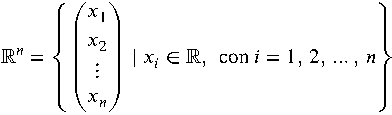
\includegraphics[page=1]{Externalizacion/C1/MatricesC1.pdf}}
    \end{matrizn}
    en donde existen dos operaciones: Dados $\mathbb{x}$, $\mathbb{y} \in \RR[n]$ con \(\mathbb{x} = \begin{pNiceMatrix}[cell-space-limits=3pt] \vphantom{^A}x_1 \\ x_2 \\ \vdots \\ x_n\vphantom{_{A_A}} \end{pNiceMatrix}\) e \(\mathbb{y} = \begin{pNiceMatrix}[cell-space-limits=3pt] \vphantom{^A}y_1 \\ y_2 \\ \vdots \\ y_n\vphantom{_{A_A}} \end{pNiceMatrix}\),
    \begin{matrizn}
        \makecell{\includegraphics[page=2]{Externalizacion/C1/MatricesC1.pdf}}
    \end{matrizn}
    A los números $x_1$, $x_2$, $\dots$, $x_n$ les llamaremos entradas o componentes de $\mathbb{x}$.
\end{definicion}

\begin{definicion}{}{}
    Sean $\mathbb{x}$, $\mathbb{y} \in \RR[n]$. Diremos que $\mathbb{x}$ e $\mathbb{y}$ son \emph{iguales} (también llamado \emph{equivalentes}), denotado por $\mathbb{x} =\mathbb{y}$, si y solo si $x_i = y_i$ para toda $i = 1, 2, \dots, n$. Es decir, si todas las entradas de $\mathbb{x}$ e $\mathbb{y}$ son iguales, entonces $\mathbb{x} = \mathbb{y}$.
\end{definicion}
\sideFigure[\label{HAJAHVSVAVVCAC}Representación geométrica de algunos ejemplos del conjunto $V$]{\vspace{4cm}
\begin{tikzpicture}
    \draw[thick,-Stealth] (-2.5,0) -- (2.5,0) node[below left] {$x$};
    \draw[thick,-Stealth] (0,-2.5) -- (0,2.5) node[below left] {$y$};
    \draw[draw={black!50}] (-2,-2) -- (2,2) node[above] {$y = x$};
    \draw[draw={black!75}] (-1,-2) -- (1,2) node[above] {$y = 2x$};
    \draw[draw={black!50}] (-2,-2/3) -- (2,2/3) node[above] {$y = \dfrac{1}{3}x$};
    \filldraw (0,0) circle (1.75pt) node[below right] {$\begin{pmatrix}
        0 \\
        0
    \end{pmatrix}$};
\end{tikzpicture}
}
\begin{examplebox}{}{}
    Sea
    $$V = \left\{ \begin{pmatrix}
        x \\
        y
    \end{pmatrix} \in \RR[2] \mid y = mx, \text{ con } m \in \RR \text{ fijo} \right\}$$
    con la suma y multiplicación por un escalar definidas en $\RR[2]$. Notemos que la expresión $y = mx$ representa una recta en el plano cartesiano con pendiente $m$ que pasa por el origen, donde $x$ y $y$ son las coordenadas de un punto y $m$ es una constante. Este conjunto admite una interpretación geométrica (vea la figura \ref{HAJAHVSVAVVCAC}). Observemos que
    $$V = \left\{ \begin{pmatrix}
        x \\
        mx
    \end{pmatrix} \in \RR[2] \mid m \in \RR \text{ fijo} \right\}.$$
    Verifiquemos entonces, los diez axiomas de un espacio vectorial. Así:
    \begin{enumerate}[label=\roman*), topsep=6pt, itemsep=0pt]
        \item Sea $\mathbb{x}$, $\mathbb{y} \in V$ con $\mathbb{x} = \begin{pmatrix}
            x \\
            mx
        \end{pmatrix}$, $\mathbb{y} = \begin{pmatrix}
            y \\
            my
        \end{pmatrix}$, entonces
        \begin{align*}
            \mathbb{x} + \mathbb{y} & = \begin{pmatrix}
                x \\
                mx
            \end{pmatrix} + \begin{pmatrix}
                y \\
                my
            \end{pmatrix} \\
            & = \begin{pmatrix}
                x + y \\
                mx + my
            \end{pmatrix} && \text{por def. de suma} \\
            & = \begin{pmatrix}
                x + y \\
                m(x + y)
            \end{pmatrix} && \text{por distributividad en $\RR$} \\
            & = \begin{pmatrix}
                \chi \\
                m\chi
            \end{pmatrix} \in V && \text{siendo $\chi = x + y$}
        \end{align*}
        Por tanto, se cumple la propiedad de cerradura.\newpage
        \item Sea $\mathbb{x}$, $\mathbb{y}$, $\mathbb{z} \in V$ con $\mathbb{x} = \begin{pmatrix}
            m \\
            mx
        \end{pmatrix}$, $\mathbb{y} = \begin{pmatrix}
            y \\
            my
        \end{pmatrix}$, $\mathbb{z} = \begin{pmatrix}
            z \\
            mz
        \end{pmatrix}$, entonces
        \begin{align*}
            \mathbb{x} + (\mathbb{y} + \mathbb{z}) & = \begin{pmatrix}
                x \\
                mx
            \end{pmatrix} + \left[ \begin{pmatrix}
                y \\
                my
            \end{pmatrix} + \begin{pmatrix}
                z \\
                mz
            \end{pmatrix} \right] \\
            & = \begin{pmatrix}
                x \\
                mx
            \end{pmatrix} + \begin{pmatrix}
                y + z \\
                my + mz
            \end{pmatrix} && \text{por def. de suma} \\
            & = \begin{pmatrix}
                x + (y + z) \\
                mx + (my + mz)
            \end{pmatrix} && \text{por def. de suma} \\
            & = \begin{pmatrix}
                (x + y) + z \\
                (mx + my) + mz
            \end{pmatrix} && \text{por asociatividad en $\RR$} \\
            & = \begin{pmatrix}
                x + y \\
                mx + my
            \end{pmatrix} + \begin{pmatrix}
                z \\
                mz
            \end{pmatrix} && \text{por def. de suma} \\
            & = \left[ \begin{pmatrix}
                x \\
                mx
            \end{pmatrix} + \begin{pmatrix}
                y \\
                my
            \end{pmatrix} \right] + \begin{pmatrix}
                z \\
                mz
            \end{pmatrix} && \text{por def. de suma} \\
            & = (\mathbb{x} + \mathbb{y}) + \mathbb{z}
        \end{align*}
        Por tanto, se cumple la asociatividad.
        \item Sea $\mathbb{x}$, $\mathbb{y} \in V$ con $\mathbb{x} = \begin{pmatrix}
            x \\
            mx
        \end{pmatrix}$, $\mathbb{y} = \begin{pmatrix}
            y \\
            my
        \end{pmatrix}$, entonces
        \begin{align*}
            \mathbb{x} + \mathbb{y} & = \begin{pmatrix}
                x \\
                mx
            \end{pmatrix} + \begin{pmatrix}
                y \\
                my
            \end{pmatrix} \\
            & = \begin{pmatrix}
                x + y \\
                mx + my
            \end{pmatrix} && \text{por def. de suma} \\
            & = \begin{pmatrix}
                y + x \\
                my + mx
            \end{pmatrix} && \text{por conmutatividad en $\RR$} \\
            & = \begin{pmatrix}
                y \\
                my
            \end{pmatrix} + \begin{pmatrix}
                x \\
                mx
            \end{pmatrix} && \text{por def. de suma} \\
            & = \mathbb{y} + \mathbb{x}
        \end{align*}
        Por tanto, se cumple la propiedad de conmutatividad.
        \item Existe $\mathbb{0} = \begin{pmatrix}
            0 \\
            m \cdot 0
        \end{pmatrix} \in V$ tal que
        $$\mathbb{x} + \mathbb{0} = \begin{pmatrix}
            x \\
            mx
        \end{pmatrix} + \begin{pmatrix}
            0 \\
            m \cdot 0
        \end{pmatrix} = \mathbb{x}.$$
        El elemento $\mathbb{0}$ pertenece al conjunto $V$ porque cumple con la condición que define a los elementos de $V$, es decir, que la segundo componente sea igual a $m$ multiplicado por el primero. Además, $\mathbb{0}$ actúa como el neutro aditivo porque,
        \begin{align*}
            \mathbb{x} + \mathbb{0} & = \begin{pmatrix}
                x \\
                mx
            \end{pmatrix} + \begin{pmatrix}
                0 \\
                m \cdot 0
            \end{pmatrix} \\
            & = \begin{pmatrix}
                x + 0 \\
                mx + m \cdot 0
            \end{pmatrix} && \text{por def. de suma} \\
            & = \begin{pmatrix}
                x \\
                mx + 0
            \end{pmatrix} && \text{por propiedad en $\RR$} \\
            & = \begin{pmatrix}
                x \\
                mx
            \end{pmatrix} && \text{por neutro aditivo en $\RR$} \\
            & = \mathbb{x}
        \end{align*}
        Por lo tanto, $\mathbb{0}$ existe en $V$ y cumple con la propiedad requerida de ser el elemento neutro para la suma en este espacio.
        \item Para cada $\mathbb{x} = \begin{pmatrix}
            x \\
            mx
        \end{pmatrix} \in V$, existe $-\mathbb{x} = \begin{pmatrix}
            -x \\
            m(-x)
        \end{pmatrix} \in V$ tal que
        $$\mathbb{x} + (-\mathbb{x}) = \begin{pmatrix}
            x \\
            mx
        \end{pmatrix} + \begin{pmatrix}
            -x \\
            m(-x)
        \end{pmatrix} = \mathbb{0}.$$
        Es claro que el elemento $-\mathbb{x}$ pertenece al conjunto $V$ porque cumple con la condición que define a los elementos de $V$, es decir, que el segundo componente sea igual a $m$ multiplicado por el primero. En este caso, para $-\mathbb{x}$, el segundo componente es $m(-x)$. Además, $-\mathbb{x}$ actúa como el opuesto aditivo de $\mathbb{x}$, ya que,
        \begin{align*}
            \mathbb{x} + (-\mathbb{x}) & = \begin{pmatrix}
                x \\
                mx
            \end{pmatrix} + \begin{pmatrix}
                -x \\
                m(-x)
            \end{pmatrix} \\
            & = \begin{pmatrix}
                x + (-x) \\
                mx + m(-x)
            \end{pmatrix} && \text{por def. de suma} \\
            & = \begin{pmatrix}
                x - x \\
                m\big(x + (-x)\big)
            \end{pmatrix} && \text{por distributividad en $\RR$} \\
            & = \begin{pmatrix}
                0 \\
                m \cdot 0
            \end{pmatrix} && \text{por inv. aditivo en $\RR$} \\
            & = \mathbb{0}
        \end{align*}
        Por tanto, se cumple la propiedad del inverso aditivo.
        \item Sea $\alpha \in \RR$ y sea $\mathbb{x} \in V$ con $\mathbb{x} = \begin{pmatrix}
            x \\
            mx
        \end{pmatrix}$, entonces
        \begin{align*}
            \alpha \cdot \mathbb{x} & = \alpha \cdot \begin{pmatrix}
                x \\
                mx
            \end{pmatrix} \\
            & = \begin{pmatrix}
                \alpha x \\
                \alpha mx
            \end{pmatrix} && \text{por def. de producto} \\
            & = \begin{pmatrix}
                (\alpha x) \\
                m(\alpha x)
            \end{pmatrix} && \text{por asociatividad en $\RR$} \\
            & = \begin{pmatrix}
                \xi \\
                m\xi
            \end{pmatrix} \in V && \text{siendo $\xi = \alpha x$}
        \end{align*}
        Por tanto, se cumple la propiedad de cerradura.
        \item Se deja como ejercicio al lector.
        \item Sea $\alpha \in \RR$ y sean $\mathbb{x}$, $\mathbb{y} \in V$ con $\mathbb{x} = \begin{pmatrix}
            x \\
            mx
        \end{pmatrix}$ e $\mathbb{y} = \begin{pmatrix}
            y \\
            my
        \end{pmatrix}$, entonces
        \begin{align*}
            \alpha \cdot (\mathbb{x} + \mathbb{y}) & = \alpha \cdot \left[ \begin{pmatrix}
                x \\
                mx
            \end{pmatrix} + \begin{pmatrix}
                y \\
                my
            \end{pmatrix} \right] \\
            & = \alpha \cdot \begin{pmatrix}
                x + y \\
                mx + my
            \end{pmatrix} && \text{por def. de suma} \\
            & = \begin{pmatrix}
                \alpha (x + y) \\
                \alpha (mx + my)
            \end{pmatrix} && \text{por def. de producto} \\
            & = \begin{pmatrix}
                \alpha x + \alpha y \\
                \alpha mx + \alpha my
            \end{pmatrix} && \text{por distributividad en $\RR$} \\
            & = \begin{pmatrix}
                \alpha x \\
                \alpha mx
            \end{pmatrix} + \begin{pmatrix}
                \alpha y \\
                \alpha my
            \end{pmatrix} && \text{por def. de suma} \\
            & = \alpha \cdot \begin{pmatrix}
                x \\
                mx
            \end{pmatrix} + \alpha \cdot \begin{pmatrix}
                y \\
                my
            \end{pmatrix} && \text{por def. de producto} \\
            & = \alpha \cdot \mathbb{x} + \alpha \cdot \mathbb{y}
        \end{align*}
        Por tanto, se cumple la distributividad con dos vectores y un escalar.
        \item Sea $\alpha$, $\beta \in \RR$ y sea $\mathbb{x} \in V$ con $\mathbb{x} = \begin{pmatrix}
            x \\
            mx
        \end{pmatrix}$, entonces
        \begin{align*}
            (\alpha + \beta) \cdot \mathbb{x} & = (\alpha + \beta) \cdot \begin{pmatrix}
                x \\
                mx
            \end{pmatrix} \\
            & = \begin{pmatrix}
                (\alpha + \beta) \cdot x \\
                (\alpha + \beta) \cdot mx
            \end{pmatrix} && \text{por def. de producto} \\
            & = \begin{pmatrix}
                \alpha x + \beta x \\
                \alpha mx + \beta mx
            \end{pmatrix} && \text{por distributividad en $\RR$} \\
            & = \begin{pmatrix}
                \alpha x \\
                \alpha mx
            \end{pmatrix} + \begin{pmatrix}
                \beta x \\
                \beta mx
            \end{pmatrix} && \text{por def. de suma} \\
            & = \alpha \cdot \mathbb{x} + \beta \cdot \mathbb{x} && \text{por def. de producto}
        \end{align*}
        Por tanto, se cumple la distributividad con dos escalares y un vector.
        \item Sea $\mathbb{x} \in V$ con $\mathbb{x} = \begin{pmatrix}
            x \\
            mx
        \end{pmatrix}$, entonces
        \begin{align*}
            1 \cdot \mathbb{x} & = 1 \cdot \begin{pmatrix}
                x \\
                mx
            \end{pmatrix} \\
            & = \begin{pmatrix}
                1 \cdot x \\
                1 \cdot mx
            \end{pmatrix} && \text{por def. de producto} \\
            & = \begin{pmatrix}
                x \\
                mx
            \end{pmatrix} && \text{por identidad multiplicactiva en $\RR$} \\
            & = \mathbb{x}
        \end{align*}
        Por tanto, se cumple la propiedad de identidad multiplicativa.
    \end{enumerate}
    Por tanto, $V$ es un espacio vectorial sobre $\RR$.
\end{examplebox}
\sideFigure[\label{UAJAJJSHSHHCGTQTTA}Representación geométrica de algunos ejemplos del conjunto $U$]{\vspace{4cm}
\begin{tikzpicture}
    \draw[thick,-Stealth] (-2.5,0) -- (2.5,0) node[below left] {$x$};
    \draw[thick,-Stealth] (0,-2.5) -- (0,2.5) node[below left] {$y$};
    \draw[draw={black!50}] (-2,-1) -- (1,2) node[above right] {$y = x + 1$};
    \draw[draw={black!75}] (-1.5,-2) node[below] {$y = 2x + 1$} -- (0.5,2);
    \draw[draw={black!50}] (-2,1/3) -- (2,5/3) node[below] {$y = \dfrac{1}{3}x + 1$};
    \filldraw (0,1) circle (2pt) node [below right] {$\begin{pmatrix} 0 \\ 1 \end{pmatrix}$};
\end{tikzpicture}
}
\begin{examplebox}{}{}
    Sea
    $$\displaystyle U = \left\{ \begin{pmatrix}
        x \\
        y
    \end{pmatrix} \in \RR[2] \mid y = mx+1, \text{ con }  m \in \RR \text{ fijo} \right\}$$
    con las operaciones de suma y multiplicación por un escalar definidas en $\RR[2]$. Demostremos que $U$ no es un espacio vectorial sobre $\RR$. Obervemos que
    $$U = \left\{ \begin{pmatrix}
        x \\
        mx + 1
    \end{pmatrix} \in \RR[2] \mid m \in \RR \text{ fijo} \right\}$$
    Así, se sigue que:
    \begin{enumerate}[label=\roman*), topsep=6pt, itemsep=0pt]
        \item Sea $\mathbb{x}$, $\mathbb{y} \in V$ con $\mathbb{x} = \begin{pmatrix}
            x \\
            mx + 1
        \end{pmatrix}$, $\mathbb{y} = \begin{pmatrix}
            y \\
            my + 1
        \end{pmatrix}$, entonces
        \begin{align*}
            \mathbb{x} + \mathbb{y} & = \begin{pmatrix}
                x \\
                mx + 1
            \end{pmatrix} + \begin{pmatrix}
                y \\
                my + 1
            \end{pmatrix} \\
            & = \begin{pmatrix}
                x + y \\
                mx + 1 + my + 1
            \end{pmatrix} && \text{por def. de suma} \\
            & = \begin{pmatrix}
                x + y \\
                m(x + y) + 2
            \end{pmatrix} && \text{por distributividad en $\RR$} \\
            & = \begin{pmatrix}
                \chi \\
                m\chi + 2
            \end{pmatrix} \notin U && \text{siendo $\chi = x + y$}
        \end{align*}
        Por tanto, no se cumple la propiedad de cerradura.
    \end{enumerate}
    Por tanto, $U$ no es un espacio vectorial sobre $\RR$. De igual forma al anterior ejemplo, $U$ admite una interpretación geométrica sencilla, vea la figura \ref{UAJAJJSHSHHCGTQTTA}.
\end{examplebox}

El siguiente ejemplo es el espacio vectorial de funciones reales en $(-\infty, \infty)$.

\newpage
\sideFigure[\label{fig:propfunc}]{
    \begin{flushleft}
        \begin{tikzpicture}
            \tikzmath{
                \c = 1.25;
                \a = \c - 1.5;
                \b = \c + 1.5;
                function f(\x) {
                    return -0.1*(\x-\c)^2 + 0.7;
			    };
                function g(\x) {
                    return 0.3*(\x-\c)^2 + 1.7;
			    };
                function h(\x) {
                    return f(\x) + g(\x);
			    };
		    };
            \draw[black,thick] plot[domain = \a:\b, samples = 120] (\x,{f(\x)});
            \draw[black!75,thick] plot[domain = \a:\b, samples = 120] (\x,{g(\x)});
            \draw[black!50,thick] plot[domain = \a:\b, samples = 120] (\x,{h(\x)});
            \draw (\c,0) -- (\c,-0.2) node[below] {$x$};
            %
            \draw[-Stealth,thick] (0,-0.5) -- (0,3.5) node[below right] {$y$};
            \draw[-Stealth,thick] (-1,0) -- (3.5,0) node[below left] {$x$};
            %
            \node[left] at (\a,{f(\a)}) {$\mathbb{f}$};
            \node[left] at (\a,{g(\a)}) {$\mathbb{g}$};
            \node[left] at (\a,{h(\a)}) {$\mathbb{f} + \mathbb{g}$};
            %
            \filldraw[black] (\c,{f(\c)}) circle (2pt);
            \filldraw[black!75] (\c,{g(\c)}) circle (2pt);
            \filldraw[black!50] (\c,{h(\c)}) circle (2pt);
            %
            \draw[black, decorate, decoration={brace,raise=5pt}, transform shape] (\c,0.05) -- node[midway, left, xshift=-7pt] {$f(x)$} (\c,{f(\c)});
            \draw[black, decorate, decoration={brace,mirror,raise=5pt}, transform shape] (\c,0.05) -- node[midway, right, xshift=7pt, yshift=3pt] {$g(x)$} (\c,{g(\c)});
            \draw[black, decorate, decoration={brace,mirror,raise=5pt}, transform shape] (2.1,0.05) -- node[midway, right, xshift=7pt] {$f(x) + g(x)$} (2.1,{h(\c)});
            \node at (0,5) {~};
        \end{tikzpicture}
        \TituloBox{\normalsize(a)}\\[3mm]
        \begin{tikzpicture}
            \tikzmath{
                \c = 1.25;
                \a = \c - 1.5;
                \b = \c + 1.5;
                function f(\x) {
                    return -0.1*(\x-\c)^2 + 0.7;
			    };
                function h(\x) {
                    return 2.5*f(\x);
			    };
		    };
            \draw[black,thick] plot[domain = \a:\b, samples = 120] (\x,{f(\x)});
            \draw[black!75,thick] plot[domain = \a:\b, samples = 120] (\x,{h(\x)});
            \draw (\c,0) -- (\c,-0.2) node[below] {$x$};
            %
            \draw[-Stealth,thick] (0,-0.5) -- (0,3.5) node[below right] {$y$};
            \draw[-Stealth,thick] (-1,0) -- (3.5,0) node[below left] {$x$};
            %
            \node[left] at (\a,{f(\a)}) {$\mathbb{f}$};
            \node[left] at (\a,{h(\a)}) {$\alpha \cdot \mathbb{f}$};
            %
            \filldraw[black] (\c,{f(\c)}) circle (2pt);
            \filldraw[black!50] (\c,{h(\c)}) circle (2pt);
            %
            \draw[black, decorate, decoration={brace,raise=5pt}, transform shape] (\c,0.05) -- node[midway, left, xshift=-7pt] {$f(x)$} (\c,{f(\c)});
            \draw[black, decorate, decoration={brace,mirror,raise=5pt}, transform shape] (\c,0.05) -- node[midway, right, xshift=7pt, yshift=3pt] {$\alpha f(x)$} (\c,{h(\c)});
        \end{tikzpicture}
        \,\\
        \TituloBox{\normalsize(b)}\\[3mm]
        \begin{tikzpicture}
            \tikzmath{
                \c = 1.25;
                \a = \c - 1.5;
                \b = \c + 1.5;
                function f(\x) {
                    return -0.1*(\x-\c)^2 + 0.7;
			    };
                function h(\x) {
                    return -1*f(\x);
			    };
		    };
            \draw[black,thick] plot[domain = \a:\b, samples = 120] (\x,{f(\x)});
            \draw[black!75,thick] plot[domain = \a:\b, samples = 120] (\x,{h(\x)});
            \draw (\c,0) -- (\c,-0.2);
            %
            \draw[black!50,thick] (\a,0) -- (3.4,0);
            \draw[-Stealth,thick] (0,-1.5) -- (0,2.5) node[below right] {$y$};
            \draw[-Stealth,thick] (3.45,0) -- (3.5,0) node[below left] {$x$};
            \draw[white] (-1,0) -- (-0.99,0);
            %
            \node[left] at (\a,{f(\a)}) {$\mathbb{f}$};
            \node[left] at (\a,{h(\a)}) {$-\mathbb{f}$};
            \node[left] at (\a,0) {$\mathbb{0}$};
            %
            \filldraw[black] (\c,{f(\c)}) circle (2pt);
            \filldraw[black!50] (\c,{h(\c)}) circle (2pt);
            %
            \draw[black, decorate, decoration={brace,raise=5pt}, transform shape] (\c,0.05) -- node[midway, left, xshift=-7pt] {$f(x)$} (\c,{f(\c)});
            \draw[black, decorate, decoration={brace,raise=5pt}, transform shape] (\c,{h(\c)}) -- node[midway, left, xshift=-7pt] {$-f(x)$} (\c,-0.05);
        \end{tikzpicture}
        \,\\
        \TituloBox{\normalsize(c)}
    \end{flushleft}
}

\begin{examplebox}{}{ejemplo5.1.8}
    Sea $V$ el conjunto de funciones con valores reales definidas en cada $x$ en el intervalo $(-\infty, \infty)$. Sean $\mathbb{f} = f(x)$ y $\mathbb{g} = g(x)$ dos funciones en $V$ y $\alpha$ un escalar, definimos
    \begin{equation}
        (\mathbb{f} + \mathbb{g})(x) = f(x) + g(x) \label{eq:sumafuncii}
    \end{equation}
    y para $\alpha$,
    \begin{equation}
        (\alpha \cdot \mathbb{f})(x) = \alpha f(x). \label{eq:prodfuncii}
    \end{equation}
    Una forma de interpretar estas operaciones es ver los valores $f(x)$ y $g(x)$ como las “componentes” de $\mathbb{f}$ y $\mathbb{g}$ en el punto $x$. En este caso, las ecuaciones \eqref{eq:sumafuncii} y \eqref{eq:prodfuncii} establecen que dos funciones se suman agregando sus componentes correspondientes, y que una función se multiplica por un escalar multiplicando cada componente por dicho escalar, exactamente como en $\RR[n]$. Esta idea se ilustra en las partes (a) y (b) de la figura \ref{fig:propfunc}. El conjunto $V$ con estas operaciones se denota por el símbolo $F(-\infty, \infty)$. Podemos demostrar que este es un espacio vectorial de la siguiente manera:
    \begin{enumerate}[label=\roman*), topsep=6pt, itemsep=0pt]
        \item El axioma de cerradura para la suma requiere que si sumamos dos funciones definidas en cada $x$ en el intervalo $(-\infty, \infty)$, entonces la suma de esas funciones también deben estar definidas en cada $x$ en el intervalo $(-\infty, \infty)$. Esto se sigue de la fórmula \eqref{eq:sumafuncii}.
        \item Sea $\mathbb{f}$, $\mathbb{g}$, $\mathbb{h} \in V$ con $\mathbb{f} = f(x)$, $\mathbb{g} = g(x)$, $\mathbb{h} = h(x)$,
        \begin{align*}
            [\mathbb{f} + (\mathbb{g} + \mathbb{h})](x) & = f(x) + (g(x) + h(x)) \\
            & = (f(x) + g(x)) + h(x) \\
            & = [(\mathbb{f} + \mathbb{g}) + \mathbb{h}](x)
        \end{align*}
        Por tanto, se cumple la asociatividad sobre la suma de funciones.
        \item Sea $\mathbb{f}$, $\mathbb{g} \in V$ con $\mathbb{f} = f(x)$, $\mathbb{g} = g(x)$,
        \begin{align*}
            (\mathbb{f} + \mathbb{g})(x) & = f(x) + g(x) \\
            & = g(x) + f(x) \\
            & = (\mathbb{g} + \mathbb{f})(x)
        \end{align*}
        Por tanto, se cumple la propiedad de conmutatividad.
        \item Existe una función $\mathbb{0}$ en $F(-\infty, \infty)$, la cual, al sumarse con cualquier otra función $\mathbb{f}$ en $F(-\infty, \infty)$, devuelve $\mathbb{f}$ como resultado. La función cuyo valor en cada punto $x$ del intervalo $(-\infty, \infty)$ es cero cumple con esta propiedad. Geométricamente, el gráfico de la función $\mathbb{0}$ es la línea que coincide con el eje $x$. De esta forma, si tenemos $\mathbb{f}$, $\mathbb{0} \in V$ con $\mathbb{f} = f(x)$, $\mathbb{0} = 0$,
        \begin{align*}
            (\mathbb{f} + \mathbb{0})(x) & = f(x) + 0 \\
            & = f(x) \\
            & = \mathbb{f}
        \end{align*}
        Por tanto, se cumple la propiedad de neutro aditivo.
        \item Para cada función $\mathbb{f}$ en $F(-\infty, \infty)$ existe una función $-\mathbb{f}$ en $F(-\infty, \infty)$, la cual, al sumarse con $\mathbb{f}$, produce la función $\mathbb{0}$. La función definida por $-\mathbb{f}(x) = -f(x)$ cumple con esta propiedad. Geométricamente, el gráfico de $-\mathbb{f}$ se obtiene reflejando el de $\mathbb{f}$ con respecto al eje $x$ (figura \ref{fig:propfunc}c). Así,
        \begin{align*}
            [\mathbb{f} + (-\mathbb{f})](x) & = f(x) + (-f(x)) \\
            & = f(x) - f(x) \\
            & = 0 \\
            & = \mathbb{0}
        \end{align*}
        Por tanto, se cumple la propiedad de inverso aditivo.
        \item Es análogo al inciso (i) y esto se sigue de la fórmula \eqref{eq:prodfuncii}.
        \item Sea $\mathbb{f}$, $\mathbb{g} \in V$ con $\mathbb{f} = f(x)$, $\mathbb{g} = g(x)$ y sea $\alpha \in \RR$,
        \begin{align*}
            [\alpha \cdot (\mathbb{f} + \mathbb{g})](x) & = \alpha (f(x) + g(x)) \\
            & = \alpha f(x) + \alpha g(x) \\
            & = (\alpha \cdot \mathbb{f})(x) + (\alpha \cdot \mathbb{g})(x) \\
            & = (\alpha \cdot \mathbb{f} + \alpha \cdot \mathbb{g})(x)
        \end{align*}
        Por tanto, se cumple la distributividad sobre la suma de vectores.
        \item Sea $\mathbb{f} \in V$ con $\mathbb{f} = f(x)$ y sea $\alpha$, $\beta \in \RR$,
        \begin{align*}
            [(\alpha + \beta) \cdot \mathbb{f}](x) & = (\alpha + \beta) f(x) \\
            & = \alpha f(x) + \beta f(x) \\
            & = (\alpha \cdot \mathbb{f})(x) + (\beta \cdot \mathbb{f})(x) \\
            & = (\alpha \cdot \mathbb{f} + \beta \cdot \mathbb{f})(x)
        \end{align*}
        Por tanto, se cumple la distributividad sobre la suma de escalares.
        \item Se deja como ejercicio al lector.
        \item Sea $\mathbb{f} \in V$ con $\mathbb{f} = f(x)$ y sea $1 \in \RR$,
        \begin{align*}
            (1 \cdot \mathbb{f})(x) & = 1 f(x) \\
            & = f(x) \\
            & = \mathbb{f}
        \end{align*}
        Por tanto, se cumple la propiedad de identidad multiplicativa.
    \end{enumerate}
    Dado que $F(-\infty, \infty)$ satisface todas las propiedades requeridas para ser un espacio vectorial, concluimos que $F(-\infty, \infty)$ es un espacio vectorial sobre $\RR$.
\end{examplebox}

Es crucial entender que no se pueden imponer arbitrariamente dos operaciones en un conjunto $V$ y esperar que se cumplan los axiomas de espacio vectorial. Por ejemplo, si $V$ es el conjunto de vectores de $\RR[n]$ con componentes positivas y se usan las operaciones estándar de $\RR[n]$, entonces $V$ no es cerrado bajo la multiplicación por escalares, ya que $(-1) \cdot \mathbb{u}$ es un vector con al menos un componente negativo, que no pertenecería a $V$.

El siguiente es un ejemplo menos evidente en el que solo uno de los diez axiomas de espacio vectorial deja de cumplirse.

\begin{examplebox}{}{}
    Sea $V = \RR[2]$ y definamos las operaciones de suma y producto escalar en $V$ de la siguiente manera: Si $\mathbb{u} = \begin{pmatrix}
        u_1 \\
        u_2
    \end{pmatrix}$, $\mathbb{v} = \begin{pmatrix}
        v_1 \\
        v_2
    \end{pmatrix}$ y si $\alpha$ es un número real cualquiera,
    $$\mathbb{u} + \mathbb{v} = \begin{pmatrix}
        u_1 + v_1 \\
        u_2 + v_2
    \end{pmatrix} \quad \text{ y } \quad \alpha \cdot \mathbb{u} = \begin{pmatrix}
        \alpha u_1 \\
        0
    \end{pmatrix}.$$
    Por ejemplo, si $\mathbb{u} = \begin{pmatrix}
        2 \\
        4
    \end{pmatrix}$, $\mathbb{v} = \begin{pmatrix*}[r]
        -3 \\
        5
    \end{pmatrix*}$ y $\alpha = 7$, entonces
    $$\mathbb{u} + \mathbb{v} = \begin{pmatrix}
        2 + (-3) \\
        4 + 5
    \end{pmatrix} = \begin{pmatrix*}[r]
        -1 \\
        9
    \end{pmatrix*} \quad \text{ y } \quad \alpha \cdot \mathbb{u} = 7 \cdot \mathbb{u} = \begin{pmatrix}
        7 \cdot 2 \\
        0
    \end{pmatrix} = \begin{pmatrix}
        14 \\ 
        0
    \end{pmatrix}.$$
    La operación de suma es la estándar en $\RR[2]$, pero el producto escalar no lo es. Los primeros nueve axiomas se cumplen, sin embargo, el axioma (x) no se cumple para ciertos vectores. Por ejemplo, si $\mathbb{u}$ es tal que $u_2 \neq 0$, entonces
    $$1 \cdot \mathbb{u} = 1 \cdot \begin{pmatrix}
        u_1 \\
        u_2
    \end{pmatrix} = \begin{pmatrix}
        1 \cdot u_1 \\
        0
    \end{pmatrix} = \begin{pmatrix}
        u_1 \\
        0
    \end{pmatrix} \neq \mathbb{u}.$$
    Por lo tanto, $V$ no es un espacio vectorial con las operaciones establecidas.
\end{examplebox}

\newpage

Nuestro siguiente ejemplo será un espacio vectorial inusual que hemos incluido para ilustrar la variedad de espacios vectoriales.

\begin{examplebox}{}{}
    Sea $V$ el conjunto de los números reales positivos, y sean $\mathbb{u} = u$ y $\mathbb{v} = v$ cualesquiera vectores (es decir, números reales positivos) en $V$. Sea $\alpha$ un escalar cualquiera. Definimos las operaciones en $V$ como
    $$\mathbb{u} + \mathbb{v} = uv \quad \text{ y } \quad \alpha \cdot \mathbb{u} = u^{\alpha}.$$
    Por ejemplo, $1 + 1 = (1)(1) = 1$ y $(2)(1) = 1^2 = 1$, lo cual resulta extraño, pero, no obstante, el conjunto $V$ con estas operaciones satisface los diez axiomas de los espacios vectoriales y, por lo tanto, es un espacio vectorial. Verificaremos algunos axiomas, y dejaremos los demás como ejercicio al lector.
    \begin{enumerate}[label=\roman*), topsep=6pt, itemsep=0pt]
        \item Dado que $\mathbb{u} = u$ y $\mathbb{v} = v$ son números reales positivos, el producto $uv$ es también un número real positivo, ya que el producto de dos números reales positivos siempre da como resultado otro número real positivo.
        \item Sea $\mathbb{u}$, $\mathbb{v} \in V$ con $\mathbb{u} = u$, $\mathbb{v} = v$,
        \begin{align*}
            \mathbb{u} + \mathbb{v} & = uv \\
            & = vu \\
            & = \mathbb{v} + \mathbb{u}
        \end{align*}
        Por tanto, se cumple la propiedad de conmutatividad.
        \item Se deja como ejercicio al lector.
        \item Sea $\mathbb{u}$, $\mathbb{0} \in V$ con $\mathbb{u} = u$, $\mathbb{0} = 1$,
        \begin{align*}
            \mathbb{u} + \mathbb{0} & = u^1 \\
            & = u \\
            & = \mathbb{u}
        \end{align*}
        Por tanto, se cumple la propiedad de neutro aditivo.
        \item Dado $\mathbb{u} = u$, existe $-\mathbb{u} = \dfrac{1}{u}$ que satisface
        \begin{align*}
            \mathbb{u} + (-\mathbb{u}) & = u \left( \frac{1}{u} \right) \\
            & = 1 \\
            & = \mathbb{0}
        \end{align*}
        Por tanto, se cumple la propiedad de inverso aditivo.
        \item Dado que $\mathbb{u} = u$ es un número real positivo, y $\alpha$ es un número real cualquiera, la operación $u^{\alpha}$ es también un número real positivo.
        \item Sea $\mathbb{u}$, $\mathbb{v} \in V$ con $\mathbb{u} = u$, $\mathbb{v} = v$ y sea $\alpha \in \RR$,
        \begin{align*}
            \alpha \cdot (\mathbb{u} + \mathbb{v}) & = (uv)^{\alpha} \\
            & = u^{\alpha} v^{\alpha} \\
            & = \alpha \cdot \mathbb{u} + \alpha \cdot \mathbb{v}
        \end{align*}
        Por tanto, se cumple la distributividad sobre la suma de vectores.
        \item Sea $\mathbb{u} \in V$ con $\mathbb{u} = u$ y sea $\alpha$, $\beta \in \RR$,
        \begin{align*}
            (\alpha + \beta) \cdot \mathbb{u} & = u^{\alpha + \beta} \\
            & = u^{\alpha} u^{\beta} \\
            & = \alpha \cdot \mathbb{u} + \beta \cdot \mathbb{u}
        \end{align*}
        Por tanto, se cumple la distributividad sobre la suma de escalares.
        \item Se deja como ejercicio al lector.
        \item Se deja como ejercicio al lector.
    \end{enumerate}
    En conclusión, aunque estas operaciones resulten inusuales, la verificación de los diez axiomas, confirma que esta estructura cumple con todos los requisitos para ser considerada un espacio vectorial sobre $\RR$.
\end{examplebox}

El siguiente ejemplo es el espacio vectorial de los polinomios con coeficientes reales, que cumple con los axiomas correspondientes.

\begin{examplebox}{}{POLIREALES}
    El conjunto de polinomios reales de grado menor o igual a $n$ se define como
    $$P_n = \left\{ a_nx^n + a_{n-1}x^{n-1} + \cdots + a_1x + a_0 \mid a_i \in \RR, \text{ para } i = 0, 1, 2, \dots, n \right\}$$
    y se expresan los elementos como
    $$p(x) = a_nx^n + a_{n-1}x^{n-1} + \cdots + a_1x + a_0$$
    En $P_n$, definimos dos operaciones: Dado $p(x) \in P_n$ y $\alpha \in \RR$,
    \begin{alignat*}{2}
        + & : & \quad P_n \times P_n & \longrightarrow P_n \\
        & & \big(p(x), q(x) \big) & \longmapsto p(x)+q(x) \\
        & \\
        \cdot & : & \quad \RR \times P_n & \longrightarrow P_n \\
        & & \big(\alpha, p(x) \big) & \longmapsto \alpha \cdot p(x)
    \end{alignat*}
    donde
    $$p(x) + q(x) = (a_n + b_n)x^n + (a_{n-1} + b_{n-1})x^{n-1} + \cdots + (a_1 + b_1)x + (a_0 + b_0)$$
    y
    $$\alpha \cdot p(x) = \alpha a_nx^n + \alpha a_{n-1}x^{n-1} + \cdots + \alpha a_1x + \alpha a_0.$$
    Entonces $P_n$ es un espacio vectorial sobre $\RR$. Es obvio que la suma de dos polinomios de grado menor o igual a $n$ es otro polinomio de grado menor o igual a $n$, por lo que se cumple el axioma (i). Las propiedades (ii) y (v) a (x) son claras. Si se define el polinomio
    $$\mathbb{0} = 0 x^n+0 x^{n-1} + \cdots + 0 x + 0,$$
    entonces $\mathbb{0} \in P_n$ y el axioma (iii) se cumple. Por último, sea
    $$-p(x) = -a_n x^n - a_{n-1} x^{n-1} - \cdots - a_1 x - a_0;$$
    se ve que el axioma (iv) se cumple, con lo que $P_n$ es un espacio vectorial real.
\end{examplebox}

Nuestro último ejemplo es el más sencillo, ya que corresponde al espacio vectorial cero. A diferencia de los ejemplos anteriores, más complejos, este caso se verifica de manera trivial, ya que solo contiene el vector nulo.

\begin{examplebox}{}{}
    Sea $W$ un conjunto que consta de un único elemento, $\mathbb{0}$, y definimos
    $$\mathbb{0} + \mathbb{0} = \mathbb{0} \quad \text{ y } \quad \alpha \cdot \mathbb{0} = \mathbb{0}$$
    para todo escalar $\alpha$. A esto lo llamamos el \emph{espacio vectorial cero}.
\end{examplebox}

\section{Subespacios vectoriales}

A menudo ocurre que algún espacio vectorial de interés está contenido dentro de un espacio vectorial más grande cuyas propiedades son conocidas. En esta sección mostraremos cómo reconocer cuándo ocurre esto, explicaremos cómo las propiedades del espacio vectorial más grande pueden usarse para obtener propiedades del espacio vectorial más pequeño, y proporcionaremos una variedad de ejemplos.

\newpage

\begin{definicion}{}{}
    Se dice que $W$ es un \emph{subespacio vectorial} de $V$ si $W$ es un subconjunto no vacío de $V$, y $W$ es un espacio vectorial, junto con las operaciones de suma entre vectores y multiplicación por un escalar definidas para $V$.
\end{definicion}

En general, para demostrar que un conjunto no vacío $W$ con dos operaciones es un espacio vectorial, se deben verificar los diez axiomas de espacio vectorial. Sin embargo, si $W$ es un subespacio de un espacio vectorial conocido $V$, entonces ciertos axiomas no necesitan ser verificados porque son “heredados” de $V$. Por ejemplo, no es necesario verificar que $\mathbb{u} + \mathbb{v} = \mathbb{v} + \mathbb{u}$ se cumple en $W$ porque se cumple para todos los vectores en $V$, incluidos los de $W$. Por otro lado, es necesario verificar que $W$ está cerrado bajo la suma y la multiplicación escalar, ya que es posible que sumar dos vectores en $W$ o multiplicar un vector en $W$ por un escalar produzca un vector en $V$ que no esté en $W$ (figura \ref{JAJJAJAJAJJQJQOOQPQZ}).
\begin{figure}[h!]
    \centering
    \begin{tikzpicture}
        \coordinate (A) at (0,2);
        \coordinate (B) at (5,0);
        \coordinate (C) at (7,1.5);
        \coordinate (D) at (2,3.5);
        %
        \draw (A) -- (B) node[above] {$V$} -- (C) -- (D) -- cycle;
        \filldraw[black!7!white] ($(C)!.78!(A)$) -- ($(D)!.78!(B)$) -- ($(A)!.78!(C)$) -- ($(B)!.78!(D)$) -- cycle;
        \draw ($(C)!.78!(A)$) -- ($(D)!.78!(B)$) node[above] {$W$} -- ($(A)!.78!(C)$) -- ($(B)!.78!(D)$) -- cycle;
        \filldraw (3.25,1.5) circle (1.5pt);
        \draw[-latex] (3.25,1.5) -- node[midway,below] {$\mathbb{v}$} (4,1.75);
        \draw[-latex] (3.25,1.5) -- node[midway,left] {$\mathbb{u}$} (2.8,2.4);
        \draw[-latex] (3.25,1.5) -- (3.55,2.65);
        \draw[dashed] (2.8,2.4) -- (3.55,2.65) -- (4,1.75);
        \draw[-latex] (2.8,2.4) -- node[midway,left] {$\alpha \mathbb{u}$} (2.4,3.2);
        \draw[thin] (3.5,2) -- (4.5,2.75) node[above] {$\mathbb{u} + \mathbb{v}$};
    \end{tikzpicture}
    \caption{Los vectores $\mathbb{u}$ y $\mathbb{v}$ están en $W$, pero los vectores $\mathbb{u} + \mathbb{v}$ y $\alpha \mathbb{u}$ no lo están}
    \label{JAJJAJAJAJJQJQOOQPQZ}
\end{figure}

\noindent Los axiomas que no son heredados por $W$ son:
\begin{itemize}
    \item \textbf{Axioma 1:} Cerradura de $W$ bajo la suma.
    \item \textbf{Axioma 4:} Existencia de un vector cero en $W$.
    \item \textbf{Axioma 5:} Existencia de un negativo en $W$ para cada vector en $W$.
    \item \textbf{Axioma 6:} Cerradura de $W$ bajo la multiplicación escalar.
\end{itemize}
Por lo tanto, estos deben ser verificados para probar que $W$ es un subespacio de $V$. Sin embargo, el siguiente teorema muestra que si los axiomas 1 y 6 se cumplen en $W$, entonces los axiomas 4 y 5 se cumplen en $W$ como consecuencia.

\begin{theorem}{}{JAJSUJGBUHBOSOIOOSK}
    Si $W$ es un conjunto de uno o más vectores en un espacio vectorial $V$, entonces $W$ es un subespacio de $V$ si y solo si se satisfacen las siguientes condiciones:
    \begin{enumerate}[label=\alph*), topsep=6pt, itemsep=0pt]
        \item Si $\mathbb{u}$ y $\mathbb{v}$ son vectores en $W$, entonces $\mathbb{u} + \mathbb{v}$ está en $W$.
        \item Si $\alpha$ es un escalar y $\mathbb{u}$ es un vector en $W$, entonces $\alpha \cdot \mathbb{u}$ está en $W$.
    \end{enumerate}

    \tcblower
    \demostracion Por definición, un subespacio es un espacio vectorial cuyos elementos pertenecen a $V$ y cuyas operaciones son las mismas que en $V$. Como $V$ es un espacio vectorial, se tiene que $W$ está cerrado bajo la suma y el producto escalar, que corresponden exactamente a las condiciones (a) y (b). Recíprocamente, supongamos que se satisfacen las condiciones (a) y (b). Dado que los axiomas (i), (ii), (iii), (vii), (viii), (ix) y (x) son heredados de $V$, solo necesitamos demostrar que los axiomas (iv) y (v) se cumplen en $W$. Para ello, sea $\mathbb{u}$ un vector cualquiera en $W$. De la condición (b) se sigue que $\alpha \cdot \mathbb{u}$ es un vector en $W$ para cualquier escalar $\alpha$. En particular, $0 \cdot \mathbb{u} = \mathbb{0}$ y $(-1) \cdot \mathbb{u} = -\mathbb{u}$ están en $W$, lo que muestra que los axiomas (iv) y (v) se cumplen en $W$. 
\end{theorem}

\begin{examplebox}{}{}
    Si $V$ es un espacio vectorial y $W = \{ \mathbb{0} \}$ es el subconjunto de $V$ que consiste únicamente en el vector cero, entonces $W$ está cerrado bajo la suma y la multiplicación por un escalar, ya que
    $$\mathbb{0} + \mathbb{0} = \mathbb{0} \quad \text{ y } \quad \alpha \cdot \mathbb{0} = \mathbb{0}$$
    para cualquier escalar $\alpha$. A $W$ lo llamamos el \emph{subespacio cero} de $V$.
\end{examplebox}

\newpage

\begin{examplebox}{}{}
    Si $W$ es una recta que pasa por el origen en $\RR[2]$ o $\RR[3]$, entonces la suma de dos vectores en la recta o la multiplicación de un vector en la recta por un escalar produce otro vector en la recta. Por lo tanto, $W$ está cerrado bajo la suma y el producto escalar (véase la figura \ref{fig:rectaEV} para una ilustración en $\RR[3]$).
    \begin{center}
        \begin{tikzpicture}
            \draw[thick] (-0.5,-0.25) -- (3.75,1.875) node[right] {$W$};
            \draw[-latex,draw={black!50},thick] (0,0) -- (1,0.5) node[above left] {$\mathbb{u}$};
            \draw[-latex,draw={black!50},thick] (1,0.5) -- (2,1) node[above left] {$\mathbb{v}$};
            \draw[-latex,draw={black!50},thick] (2,1) -- (3,1.5) node[above left] {$\mathbb{u} + \mathbb{v}$};
            \draw[-Stealth,thick] (0,0) -- (0,3) node[below right] {$y$};
            \draw[-Stealth,thick] (0,0) -- (4.2,0) node[below left] {$x$};
            \draw[-Stealth,thick] (0,0) -- (-0.65,-0.9) node[above left] {$z$};
        \end{tikzpicture}
        \hfill
        \begin{tikzpicture}
            \draw[thick] (-0.5,-0.25) -- (3.75,1.875) node[right] {$W$};
            \draw[-latex,draw={black!50},thick] (0,0) -- (1,0.5) node[above left] {$\mathbb{u}$};
            \draw[-latex,draw={black!50},thick] (1,0.5) -- (2.5,1.25) node[above left] {$\alpha \cdot \mathbb{u}$};
            \draw[-Stealth,thick] (0,0) -- (0,3) node[below right] {$y$};
            \draw[-Stealth,thick] (0,0) -- (4.2,0) node[below left] {$x$};
            \draw[-Stealth,thick] (0,0) -- (-0.65,-0.9) node[above left] {$z$};
        \end{tikzpicture}
        
        \TituloBox{(a)} $W$ es cerrado bajo la suma \hfill \TituloBox{(b)} $W$ es cerrado bajo el producto escalar\captionsetup*[figure]{hypcap=false}
        \captionof{figure}{Los vectores $\mathbb{u} + \mathbb{v}$ y $\alpha \cdot \mathbb{u}$ están en la misma recta que $\mathbb{u}$ y $\mathbb{v}$}\label{fig:rectaEV}
    \end{center}
\end{examplebox}

\begin{examplebox}{}{}
    Si $\mathbb{u}$ y $\mathbb{v}$ son vectores en un plano $W$ que pasa por el origen en $\RR[3]$, entonces es evidente geométricamente que $\mathbb{u} + \mathbb{v}$ y $\alpha \cdot \mathbb{u}$ también pertenecen al mismo plano $W$ para cualquier escalar $\alpha$ (figura \ref{fig:planoEV}). Por lo tanto, $W$ está cerrado bajo la suma y el producto escalar.
    \begin{center}
        \begin{tikzpicture}
            \filldraw[black!7!white] (4.25,3) -- (0.75,3) -- (-0.25,-1) -- (3.25,-1) -- cycle;
            \draw[dashed] (1,2) -- (3,2.5) -- (2,0.5);
            \draw[-latex,draw={black!50},thick] (0,0) -- (2,0.5) node[below] {$\mathbb{u}$};
            \draw[-latex,draw={black!50},thick] (0,0) -- (3,0.75) node[below] {~~$\alpha \cdot \mathbb{u}$};
            \draw[-latex,draw={black!50},thick] (0,0) -- (1,2) node[above left] {$\mathbb{v}$};
            \draw[-latex,draw={black!50},thick] (0,0) -- (3,2.5) node[above left] {$\mathbb{u} + \mathbb{v}$};
            \draw[-Stealth,thick] (0,0) -- (0,3.5) node[below right] {$y$};
            \draw[-Stealth,thick] (0,0) -- (4.2,0) node[below left] {$x$};
            \draw[-Stealth,thick] (0,0) -- (-0.65,-0.9) node[above left] {$z$};
            \node[above left] at (3.25,-1) {$W$};
        \end{tikzpicture}
        \captionsetup*[figure]{hypcap=false}
        \captionof{figure}{Los vectores $\mathbb{u} + \mathbb{v}$ y $\alpha \cdot \mathbb{u}$ están en el mismo plano que $\mathbb{u}$ y $\mathbb{v}$}\label{fig:planoEV}
    \end{center}
\end{examplebox}

La tabla \ref{tab:subespR23} a continuación presenta una lista de los subespacios de $\RR[2]$ y $\RR[3]$ que hemos encontrado hasta ahora.
\begin{table}[H]
    \centering
    \begin{NiceTabular}{ll}[cell-space-limits=2pt]
        \CodeBefore
        \rowcolor{black!20!white}{1}
        \Body
        \toprule
        Subespacios de $\RR[2]$ & Subespacios de $\RR[3]$ \\
        \midrule
        $\bullet$\quad $\{ \mathbb{0} \}$ & $\bullet$\quad $\{ \mathbb{0} \}$ \\
        $\bullet$\quad Rectas que pasan por el origen & $\bullet$\quad Rectas que pasan por el origen \\
        $\bullet$\quad $\RR[2]$ & $\bullet$\quad Planos que pasan por el origen \\
        & $\bullet$\quad $\RR[3]$ \\
        \bottomrule
    \end{NiceTabular}
    \caption{Subespacios vectoriales de $\RR[2]$ y $\RR[3]$}
    \label{tab:subespR23}
\end{table}

En los ejemplos anteriores, hemos visto subespacios vectoriales en los espacios $\RR[2]$ y $\RR[3]$. Estos subespacios son fundamentales para comprender las propiedades estructurales de los espacios vectoriales. A continuación, daremos un ejemplo que ilustra cómo el conjunto de funciones continuas, bajo ciertas operaciones, también forma un subespacio.

\begin{examplebox}{}{EJEMPLOINI}
    Existe un teorema en cálculo que establece que la suma de funciones continuas es continua y que una constante multiplicada por una función continua también es continua. En lenguaje vectorial, el conjunto de funciones continuas en $(-\infty, \infty)$ es un subespacio de $F(-\infty, \infty)$. Denotaremos este subespacio como $C(-\infty, \infty)$.
\end{examplebox}

\newpage

\begin{examplebox}{}{}
    Una función con una derivada continua se dice que es \emph{continuamente diferenciable}. Existe un teorema en cálculo que establece que la suma de dos funciones continuamente diferenciables es continuamente diferenciable y que una constante multiplicada por una función continuamente diferenciable también es continuamente diferenciable. Por lo tanto, las funciones que son continuamente diferenciables en $(-\infty, \infty)$ forman un subespacio de $F(-\infty, \infty)$. Denotaremos este subespacio por $C^1(-\infty, \infty)$, donde el superíndice enfatiza que las primeras derivadas son continuas. Para llevar esto un paso más allá, el conjunto de funciones con $m$ derivadas continuas en $(-\infty, \infty)$ es un subespacio de $F(-\infty, \infty)$, al igual que el conjunto de funciones con derivadas de todos los órdenes en $(-\infty, \infty)$. Denotaremos estos subespacios por $C^m(-\infty, \infty)$ y $C^\infty(-\infty, \infty)$, respectivamente.
\end{examplebox}

\begin{examplebox}{}{}
    Recordemos que un \emph{polinomio} es una función que puede expresarse en la forma
    $$p(x) = a_0 + a_1x + \cdots + a_nx^n$$
    donde $a_0, a_1, \dots, a_n$ son constantes. Es evidente que la suma de dos polinomios es un polinomio y que una constante multiplicada por un polinomio también es un polinomio. Por lo tanto, el conjunto $W$ de todos los polinomios es un subespacio de $F(-\infty, \infty)$. Este espacio se denota por $P_\infty$.
\end{examplebox}

\begin{examplebox}{}{EJEMPLOFIN}
    Recordemos que el grado de un polinomio es la mayor potencia de la variable que aparece con un coeficiente distinto de cero. No es cierto que el conjunto $W$ de polinomios de grado exacto $n$ sea un subespacio de $F(-\infty, \infty)$ porque ese conjunto no está cerrado bajo la suma. Por ejemplo, los polinomios
    $$1 + 2x + 3x^2 \quad \text{ y } \quad 5 + 7x - 3x^2$$
    tienen grado $2$, pero su suma tiene grado $1$. Sin embargo, para cada entero no negativo $n$, el conjunto de polinomios de grado menor o igual a $n$ forma un subespacio de $F(-\infty, \infty)$, ya que está cerrado bajo la suma y multiplicación por un escalar.
\end{examplebox}

En nuestros ejemplos anteriores consideramos funciones que estaban definidas en todos los puntos del intervalo $(-\infty, \infty)$. A veces querremos considerar funciones que están definidas únicamente en algún subintervalo de $(-\infty, \infty)$, como el intervalo cerrado $[a, b]$ o el intervalo abierto $(a, b)$. En tales casos, realizaremos un cambio de notación apropiado. Por ejemplo, $C[a, b]$ es el espacio de funciones continuas en $[a, b]$, y $C(a, b)$ es el espacio de funciones continuas en $(a, b)$.

En cálculo se demuestra que los polinomios son funciones continuas y tienen derivadas continuas de todos los órdenes en $(-\infty, \infty)$. Por lo tanto, se deduce que $P_\infty$ no solo es un subespacio de $F(-\infty, \infty)$, como se observó anteriormente, sino que también es un subespacio de $C^\infty(-\infty, \infty)$. Dejamos al lector la tarea de convencerse de que los espacios vectoriales discutidos en los ejemplos \ref{examplebox:EJEMPLOINI} a \ref{examplebox:EJEMPLOFIN} están “anidados” unos dentro de otros, como se ilustra en la figura \ref{JAJAIQPAPOAOSOOAKJS}.
\begin{figure}[h!]
    \centering
    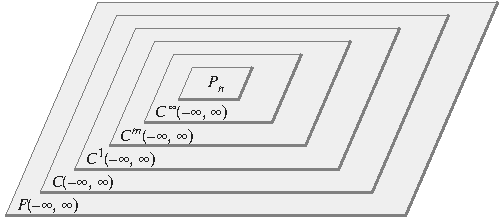
\includegraphics[width=\textwidth]{Images/Capitulo1/AnidadosBN.pdf}
    \caption{Jerarquía de espacios funcionales por diferenciabilidad}
    \label{JAJAIQPAPOAOSOOAKJS}
\end{figure}

\newpage

\begin{theorem}{}{intersubsV}
    Si $W_1, W_2, \dots, W_r$ son subespacios de un espacio vectorial $V$, entonces la intersección de estos subespacios también es un subespacio de $V$.

    \tcblower
    \demostracion Sea $W = W_1 \cap W_2 \cap \cdots \cap W_r$. Este conjunto no es vacío porque cada uno de estos subespacios contiene el vector cero de $V$, y por lo tanto, también lo hace su intersección. Así, queda por demostrar que $W$ está cerrado bajo la suma y la multiplicación por escalares. Para demostrar la cerradura bajo la suma, sean $\mathbb{u}$ y $\mathbb{v}$ vectores en $W$. Dado que $W$ es la intersección de $W_1, W_2, \dots, W_r$, se deduce que $\mathbb{u}$ y $\mathbb{v}$ también pertenecen a cada uno de estos subespacios. Además, como estos subespacios están cerrados bajo la suma y la multiplicación por escalares, también contienen los vectores $\mathbb{u} + \mathbb{v}$ y $\alpha \cdot \mathbb{u}$ para todo escalar $\alpha$, y por lo tanto, su intersección $W$ también los contiene. Esto prueba que $W$ está cerrado bajo la suma y la multiplicación por escalares.
\end{theorem}

\section{Conjuntos generadores}

\begin{definicion}{}{}
    Sea $V$ un espacio vectorial sobre $K$. Si $\mathbb{u}$ es un vector en un espacio vectorial $V$, entonces se dice que $\mathbb{u}$ es una \emph{combinación lineal} de los vectores $\mathbb{v}_1, \mathbb{v}_2, \dots, \mathbb{v}_n$ en $V$ si $\mathbb{u}$ puede expresarse en la forma
    $$\mathbb{u} = k_1 \mathbb{v}_1 + k_2 \mathbb{v}_2 + \cdots + k_n \mathbb{v}_n,$$
    donde $k_1, k_2, \dots, k_n$ son escalares. Estos escalares se denominan los \emph{coeficientes} de la combinación lineal.
\end{definicion}

Si $n = 1$, entonces la expresión de la anterior definición tiene la forma
$$\mathbb{w} = k_1\mathbb{v}_1,$$
en cuyo caso la combinación lineal es simplemente un múltiplo escalar de $\mathbb{v}_1$.

\begin{theorem}{}{CONMAPEQ}
    Sea $V$ un espacio vectorial sobre $K$. Si $S = \{\mathbb{v}_1, \mathbb{v}_2, \dots, \mathbb{v}_n\}$ es un conjunto no vacío de vectores en $V$, entonces:
    \begin{enumerate}[label=\alph*), topsep=6pt, itemsep=0pt]
        \item El conjunto $W$ de todas las combinaciones lineales posibles de los vectores en $S$ es un subespacio de $V$.
        \item El conjunto $W$ en el inciso anterior, es el subespacio más pequeño de $V$ que contiene a todos los vectores en $S$, en el sentido de que cualquier otro subespacio que contenga esos vectores también contiene a $W$.
    \end{enumerate}

    \tcblower
    \demostracion
    \begin{enumerate}[label=\alph*), topsep=6pt, itemsep=0pt]
        \item Sea $W$ el conjunto de todas las combinaciones lineales posibles de los vectores en $S$. Debemos demostrar que $W$ está cerrado bajo la suma y la multiplicación por escalares. Para demostrar la cerradura bajo la suma, sean
        $$\mathbb{x}_1 = a_1\mathbb{v}_1 + a_2\mathbb{v}_2 + \cdots + a_n\mathbb{v}_n \quad \text{ y } \quad \mathbb{x}_2 = b_1\mathbb{v}_1 + b_2\mathbb{v}_2 + \cdots + b_n\mathbb{v}_n$$
        dos vectores en $W$. Se deduce que su suma puede escribirse como
        $$\mathbb{x}_1 + \mathbb{x}_2 = (a_1 + b_1) \mathbb{v}_1 + (a_2 + b_2) \mathbb{v}_2 + \cdots + (a_n + b_n) \mathbb{v}_n,$$
        que es una combinación lineal de los vectores en $S$. Por lo tanto, $W$ está cerrado bajo la suma. Se deja como ejercicio al lector la demostración de que $W$ también está cerrado bajo la multiplicación por escalares y, por ende, es un subespacio de $V$.
        \item Sea $W'$ cualquier subespacio de $V$ que contiene a todos los vectores en $S$. Dado que $W'$ está cerrado bajo la suma y la multiplicación por escalares, contiene todas las combinaciones lineales de los vectores en $S$ y, por ende, contiene a $W$.
    \end{enumerate}
\end{theorem}

\newpage

\begin{definicion}{}{PRIM}
    Se dice que los vectores $\mathbb{v}_1, \mathbb{v}_2, \dots, \mathbb{v}_n$ de un espacio vectorial $V$ \emph{generan} a $V$ si todo vector en $V$ se puede escribir como una combinación lineal de los mismos. Es decir, para todo $\mathbb{v} \in V$ existen escalares $a_1, a_2, \dots, a_n$ tales que
    $$\mathbb{v} = a_1\mathbb{v}_1 + a_2\mathbb{v}_2 + \cdots + a_n\mathbb{v}_n.$$
\end{definicion}

\begin{examplebox}{}{vectores_unitarios_generaRn}
    Los vectores unitarios estándar en $\RR[n]$ son
    \begin{matrizn}
        \makecell{\includegraphics[page=3]{Externalizacion/C1/MatricesC1.pdf}}
    \end{matrizn}
    Estos vectores generan $\RR[n]$ ya que cualquier vector en $\RR[n]$ se puede expresar como
    $$\mathbb{v} = v_1 \mathbb{e}_1 + v_2 \mathbb{e}_2 + \dots + v_n \mathbb{e}_n$$
    lo cual es una combinación lineal de $\mathbb{e}_1, \mathbb{e}_2, \dots, \mathbb{e}_n$. Así, por ejemplo, los vectores
    \begin{matrizn}
        \makecell{\includegraphics[page=4]{Externalizacion/C1/MatricesC1.pdf}}
    \end{matrizn}
    generan $\RR[3]$ ya que cualquier vector se puede expresar como
    \begin{matrizn}
        \makecell{\includegraphics[page=5]{Externalizacion/C1/MatricesC1.pdf}}
    \end{matrizn}
\end{examplebox}

\begin{definicion}{}{SEGU}
    El \emph{espacio generado} por $\{\mathbb{v}_1, \mathbb{v}_2, \dots, \mathbb{v}_k\}$ es el conjunto de combinaciones lineales $\mathbb{v}_1, \mathbb{v}_2, \dots, \mathbb{v}_k$. Es decir,
    $$\Gen (\{\mathbb{v}_1, \mathbb{v}_2, \dots, \mathbb{v}_k\}) = \{\mathbb{v} \mid \mathbb{v} = a_1\mathbb{v}_1 + a_2\mathbb{v}_2 + \dots + a_k\mathbb{v}_k\}$$
    donde $a_1, a_2, \dots, a_k$ son escalares arbitrarios.
\end{definicion}

En las definiciones \ref{definicion:PRIM} y \ref{definicion:SEGU} se utilizaron dos términos diferentes: “genera” y “espacio generado”. Se hace hincapié en que un conjunto de vectores $\mathbb{v}_1, \mathbb{v}_2, \dots, \mathbb{v}_n$ \emph{genera} a $V$ (que es un verbo) si todo vector en $V$ se puede escribir como una combinación lineal de $\mathbb{v}_1, \mathbb{v}_2, \dots, \mathbb{v}_n$. Por otro lado, el \emph{espacio generado} (que es un sustantivo) por los $n$ vectores $\mathbb{v}_1, \mathbb{v}_2, \dots, \mathbb{v}_k$ es el conjunto de combinaciones lineales de estos vectores. Estos dos conceptos son diferentes, aún cuando los términos se parezcan. Por ejemplo, si consideramos $V = \RR[3]$,
\begin{itemize}
    \item Definición \ref{definicion:PRIM}: $\{\mathbb{e}_1, \mathbb{e}_2, \mathbb{e}_3\}$ es un conjunto generador de $V$ porque cualquier vector en $\RR[3]$ se puede escribir como combinación lineal de estos vectores.
    \item Definición \ref{definicion:SEGU}: Si tomamos $\{\mathbb{e}_1, \mathbb{e}_2\}$, el espacio generado es el subespacio $\Gen (\{\mathbb{e}_1, \mathbb{e}_2\})$, que es un plano en $\RR[3]$.
\end{itemize}
La diferencia está en que la definición \ref{definicion:PRIM} cubre el espacio completo, mientras que la \ref{definicion:SEGU} describe subespacios.

\begin{examplebox}{}{POLIGENERA}
    Los polinomios $1, x, x^2, \dots, x^n$ generan el espacio vectorial $P_n$ definido en el ejemplo \ref{examplebox:POLIREALES}, ya que cada polinomio $\mathbb{p}$ en $P_n$ puede escribirse como
    $$\mathbb{p} = a_0 + a_1x + \cdots + a_nx^n,$$
    que es una combinación lineal de $1, x, x^2, \dots, x^n$. Podemos denotar esto como
    $$P_n = \Gen\left(\left\{1, x, x^2, \dots, x^n\right\}\right).$$
\end{examplebox}

\newpage

\begin{examplebox}{}{}
    Sea $V = \RR[3]$ un espacio vectorial sobre $\RR$. Por el teorema \ref{theorem:CONMAPEQ}, se tiene que
    \begin{matriz}
        \makecell{\includegraphics[page=6]{Externalizacion/C1/MatricesC1.pdf}} \label{ec21}
    \end{matriz}
    es un subespacio de $\RR[3]$. Esto implica que $W$ está generado por las combinaciones lineales de los vectores dados. De la ecuación \eqref{ec21}, podemos expresar $W$ como
    \begin{matrizn}
        \makecell{\includegraphics[page=7]{Externalizacion/C1/MatricesC1.pdf}}
    \end{matrizn}
    De esta forma, las coordenadas de un vector genérico en $W$ se pueden describir en términos de los parámetros $\alpha$ y $\beta$ como
    $$\begin{aligned}
        x & = \alpha \\
        y & = \alpha + \beta \\
        z & = \beta
    \end{aligned} \quad \text{con } \alpha, \beta \in \RR$$
    Esto representa la forma paramétrica de un plano en $\RR[3]$. Ahora, eliminemos los parámetros $\alpha$ y $\beta$ para obtener la ecuación implícita del plano. De las expresiones para $y$ y $z$, tenemos
    $$y = x + z \Longrightarrow x - y + z = 0.$$
    Si tomamos los vectores $\mathbb{v_1}$ y $\mathbb{v_2}$ respectivamente que generan al subespacio $W$, geométricamente tenemos que
    \begin{center}
        \begin{tikzpicture}
            \begin{axis}[width=11.4cm,height=11.4cm,
            xlabel=$x$, ylabel=$y$, zlabel=$z$,
            xmin=-4.9, xmax=4.9,
            ymin=-4.9, ymax=4.9,
            zmin=-4.9, zmax=4.9,
            axis lines=center,
            axis line style={-Stealth},
            ticks=none,
            ]
                \fill[gray,opacity=0.1] (xyz cs:x=-4.9,y=-4.9,z=0) -- (xyz cs:x=4.9,y=-4.9,z=0) -- (xyz cs:x=4.9,y=4.9,z=0) --  (xyz cs:x=-4.9,y=4.9,z=0) -- cycle;
                \fill[gray!70,opacity=0.2] (xyz cs:x=-4.9,y=-4.9,z=-4.9) -- (xyz cs:x=4.9,y=4.9,z=-4.9) -- (xyz cs:x=4.9,y=4.9,z=4.9) --  (xyz cs:x=-4.9,y=-4.9,z=4.9) -- cycle;
                
                \draw[dash pattern=on 3pt off 3pt] (2,2,0) -- (2,4,2) -- (0,2,2);
                
                \draw[-latex,dash pattern=on 3pt off 3pt] (1,1,0) -- (2,2,0) node[below] {$\alpha\mathbb{v}_1$};
                \draw[-latex] (0,0,0) -- (1,1,0) node[below]{$\mathbb{v}_1$};

                \draw[-latex,dash pattern=on 3pt off 3pt] (0,1,1) -- (0,2,2) node[left] {$\beta\mathbb{v}_2$};
                \draw[-latex] (0,0,0) -- (0,1,1) node[left]{$\mathbb{v}_2$};

                \draw[-latex,thick] (0,0,0) -- (2,4,2) node[right]{$\alpha\mathbb{v}_1 + \beta\mathbb{v}_2$};
                
                \fill[gray,opacity=0.4] (xyz cs:x=-4.9,y=-4.9,z=0) -- (xyz cs:x=4.9,y=-4.9,z=0) -- (xyz cs:x=4.9,y=4.9,z=0) -- cycle;
            \end{axis}
        \end{tikzpicture}
        \captionsetup*[figure]{hypcap=false}%
        \captionof{figure}{Representación del plano $x - y + z = 0$}
    \end{center}
    Por lo tanto, el subespacio $W$ es el plano en $\RR[3]$ definido por la ecuación implícita
    $$x - y + z = 0.$$
    Esto demuestra que $W$ es efectivamente un subespacio vectorial y, además, está contenido en el plano descrito.
\end{examplebox}

\newpage

\section{Conjuntos linealmente independientes}

\begin{definicion}{}{}
    Sea $V$ un espacio vectorial sobre $K$. Un subconjunto $S$ del espacio vectorial $V$ se llama \emph{linealmente dependiente} si existen vectores distintos $\mathbb{v}_1$, $\mathbb{v}_2$, $\dots$, $\mathbb{v}_n$ en $S$ y $a_1$, $a_2$, $\dots$, $a_n$ en $K$ no todos $0$ tales que
    $$a_1 \mathbb{v}_1 + a_2 \mathbb{v}_2 + \cdots + a_n \mathbb{v}_n = \mathbb{0}.$$
    En este caso también decimos que los vectores de $S$ son linealmente dependientes. En caso contrario, decimos que los vectores son \emph{linealmente independientes} y por tanto, $S$ también es linealmente independiente.
\end{definicion}

\begin{theorem}{}{licombinacion_lineal}
    Los vectores no nulos $\mathbb{v}_1, \mathbb{v}_2, \dots, \mathbb{v}_k$ en un espacio vectorial $V$, son linealmente dependientes si, y solo si uno de los vectores $\mathbb{v}_j$, con $j \geq 2$, es una combinación lineal de los vectores que lo preceden $\mathbb{v}_1, \mathbb{v}_2, \dots, \mathbb{v}_{j-1}$.

    \tcblower
    \demostracion Si $\mathbb{v}_j$ es una combinación lineal de $\mathbb{v}_1, \mathbb{v}_2, \dots, \mathbb{v}_{j-1}$,
    $$\mathbb{v}_j = c_1 \mathbb{v}_1 + c_2 \mathbb{v}_2 + \cdots + c_{j-1} \mathbb{v}_{j-1},$$
    entonces
    $$c_1 \mathbb{v}_1 + c_2 \mathbb{v}_2 + \cdots + c_{j-1} \mathbb{v}_{j-1} + (-1) \mathbb{v}_j + 0 \mathbb{v}_{j+1} + \cdots + 0 \mathbb{v}_n = \mathbb{0}.$$
    Como por lo menos uno de los coeficientes es diferente de cero, $\mathbb{v}_1, \mathbb{v}_2, \dots, \mathbb{v}_n$ son linealmente dependientes. Supongamos ahora que $\mathbb{v}_1, \mathbb{v}_2, \dots, \mathbb{v}_n$ son linealmente dependientes. Entonces existen escalares $c_1, c_2, \dots, c_n$, no todos cero, tales que
    $$c_1 \mathbb{v}_1 + c_2 \mathbb{v}_2 + \cdots + c_n \mathbb{v}_n = \mathbb{0}.$$
    Sea $j$ el mayor subíndice para el cual $c_j \neq 0$. Si $j > 1$, entonces
    $$\mathbb{v}_j = - \left( \frac{c_1}{c_j} \right) \mathbb{v}_1 - \left( \frac{c_2}{c_j} \right) \mathbb{v}_2 - \cdots - \left( \frac{c_{j-1}}{c_j} \right) \mathbb{v}_{j-1}.$$
    Si $j = 1$, entonces $c_1 \mathbb{v}_1 = \mathbb{0}$, lo que implica que $\mathbb{v}_1 = \mathbb{0}$, contradiciendo la hipótesis de que ninguno de los vectores es el vector cero. Por lo tanto, uno de los vectores $\mathbb{v}_j$ es una combinación lineal de los vectores que lo preceden $\mathbb{v}_1, \mathbb{v}_2, \dots, \mathbb{v}_{j-1}$.
\end{theorem}

\begin{corollary}{}{}
    Dos vectores en un espacio vectorial son linealmente dependientes si y solo si uno de ellos es un múltiplo escalar del otro.
\end{corollary}

\begin{examplebox}{}{IAIAIKAJSJSKJHQUQUQUJWJS}
    Consideremos el espacio vectorial $\RR[3]$ y los vectores
    \begin{matrizn}
        \makecell{\includegraphics[page=8]{Externalizacion/C1/MatricesC1.pdf}}
    \end{matrizn}
    Notemos que
    $$\mathbb{v}_1 + \mathbb{v}_2 + 0\mathbb{v}_3 - \mathbb{v}_4 = \mathbb{0},$$
    es decir, $\mathbb{v}_1$, $\mathbb{v}_2$, $\mathbb{v}_3$ y $\mathbb{v}_4$ son linealmente dependientes. En este caso,
    $$\mathbb{v}_4 = \mathbb{v}_1 + \mathbb{v}_2.$$
\end{examplebox}

En otras palabras, si $S$ es un conjunto de dos o más vectores en $V$, se dice que es \emph{linealmente independiente} si ningún vector en $S$ puede expresarse como una combinación lineal de los demás. En caso contrario, donde al menos uno de los vectores puede escribirse como combinación lineal de los demás, el conjunto $S$ se considera \emph{linealmente dependiente}, según el precedente teorema y corolario.\infoBulle{El teorema \ref{theorem:licombinacion_lineal} no dice que en un conjunto de vectores linealmente dependientes todo vector $\mathbb{v}$ del conjunto es una combinación lineal de los vectores que le preceden. En el ejemplo \ref{examplebox:IAIAIKAJSJSKJHQUQUQUJWJS}, también se cumple que $\mathbb{v}_1 + 2\mathbb{v}_2 + \mathbb{v}_3 + 0\mathbb{v}_4 = \mathbb{0}$. Sin embargo, no podemos despejar a $\mathbb{v}_4$ para expresarlo como combinación lineal de $\mathbb{v}_1$, $\mathbb{v}_2$ y
$\mathbb{v}_3$, puesto que su coeficiente es cero.}

\newpage

La independencia lineal tiene interpretaciones geométricas útiles en $\RR[2]$ y $\RR[3]$. Dos vectores en $\RR[2]$ o $\RR[3]$ son linealmente independientes si y solo si no están sobre la misma recta cuando tienen sus puntos iniciales en el origen. De lo contrario, uno sería un múltiplo escalar del otro (figura \ref{fig:linealDR2R3}).
\begin{figure*}[h!]
    \centering
    \subfloat[Linealmente dependientes]{
        \begin{tikzpicture}
            \draw[thick] (-0.75,-0.5625) -- (3,2.25);
            \draw[-latex,draw={black!50},thick] (0,0) -- (1.5,1.125) node[above left] {$\mathbb{v}_1$};
            \draw[-latex,draw={black!50},thick] (1.5,1.125) -- (2.25,1.6875) node[above left] {$\mathbb{v}_2$};
            \draw[-Stealth,thick] (0,0) -- (0,3) node[below right] {$z$};
            \draw[-Stealth,thick] (0,0) -- (3.5,0) node[below left] {$y$};
            \draw[-Stealth,thick] (0,0) -- (-1,-1.384) node[above left] {$x$};
        \end{tikzpicture}
    } \hfill
    \subfloat[Linealmente dependientes]{
        \begin{tikzpicture}
            \draw[thick] (-1,-0.75) -- (3,2.25);
            \draw[-latex,draw={black!50},thick] (0,0) -- (1.5,1.125) node[above left] {$\mathbb{v}_1$};
            \draw[-latex,draw={black!50},thick] (0,0) -- (-0.75,-0.5625) node[above,yshift=4pt] {$\mathbb{v}_2$};
            \draw[-Stealth,thick] (0,0) -- (0,3) node[below right] {$z$};
            \draw[-Stealth,thick] (0,0) -- (3.5,0) node[below left] {$y$};
            \draw[-Stealth,thick] (0,0) -- (-1,-1.384) node[above left] {$x$};
        \end{tikzpicture}
    } \hfill
    \subfloat[Linealmente independientes]{
        \begin{tikzpicture}
            \draw[-latex,draw={black!50},thick] (0,0) -- (1.0242,1.5702) node[above left] {$\mathbb{v}_1$};
            \draw[-latex,draw={black!50},thick] (0,0) -- (1.0766,0.3265) node[above left] {$\mathbb{v}_2$};
            \draw[-Stealth,thick] (0,0) -- (0,3) node[below right] {$z$};
            \draw[-Stealth,thick] (0,0) -- (3.5,0) node[below left] {$y$};
            \draw[-Stealth,thick] (0,0) -- (-1,-1.384) node[above left] {$x$};
        \end{tikzpicture}
    }
    \caption{}
    \label{fig:linealDR2R3}
\end{figure*}

Tres vectores en $\RR[3]$ son linealmente independientes si y solo si no están sobre el mismo plano cuando tienen sus puntos iniciales en el origen. De lo contrario, al menos uno sería una combinación lineal de los otros dos (figura \ref{fig:linealDR3}).
\begin{figure*}[h!]
    \centering
    \subfloat[Linealmente dependientes]{
        \begin{tikzpicture}
            \filldraw[black!7!white] (3.75,2.5) -- (0.75,2.5) -- (-0.25,-1) -- (2.75,-1) -- cycle;
            \draw[-latex,draw={black!50},thick] (0,0) -- (1,-0.6) node[above right] {$\mathbb{v}_1$};
            \draw[-latex,draw={black!50},thick] (0,0) -- (1.5,0.75) node[above] {$\mathbb{v}_2$};
            \draw[-latex,draw={black!50},thick] (0,0) -- (2,2.25) node[left,xshift=-4pt] {$\mathbb{v}_3$};
            \draw[-Stealth,thick] (0,0) -- (0,3) node[below right] {$z$};
            \draw[-Stealth,thick] (0,0) -- (3.5,0) node[below left] {$y$};
            \draw[-Stealth,thick] (0,0) -- (-1,-1.384) node[above left] {$x$};
        \end{tikzpicture}
    } \hfill
    \subfloat[Linealmente dependientes]{
        \begin{tikzpicture}
            \filldraw[black!7!white] (3.75,2.5) -- (0.75,2.5) -- (-0.25,-1) -- (2.75,-1) -- cycle;
            \draw[-latex,draw={black!50},thick] (0,0) -- (1,-0.6) node[above right] {$\mathbb{v}_1$};
            \draw[-latex,draw={black!50},thick] (0,0) -- (1,1.125) node[left,xshift=-4pt] {$\mathbb{v}_2$};
            \draw[-latex,draw={black!50},thick] (0,0) -- (2,2.25) node[left,xshift=-4pt] {$\mathbb{v}_3$};
            \draw[-Stealth,thick] (0,0) -- (0,3) node[below right] {$z$};
            \draw[-Stealth,thick] (0,0) -- (3.5,0) node[below left] {$y$};
            \draw[-Stealth,thick] (0,0) -- (-1,-1.384) node[above left] {$x$};
        \end{tikzpicture}
    } \hfill
    \subfloat[Linealmente independientes]{
        \begin{tikzpicture}
            \filldraw[black!7!white] (3.75,2.5) -- (0.75,2.5) -- (-0.25,-1) -- (2.75,-1) -- cycle;
            \draw[-latex,draw={black!50},thick] (0,0) -- (1,-0.6) node[above right] {$\mathbb{v}_3$};
            \draw[-latex,draw={black!50},thick] (0,0) -- (1.5,0.75) node[above] {$\mathbb{v}_2$};
            \draw[-latex,draw={black!50},thick] (0,0) -- (1.5,2.8) node[left,xshift=-4pt] {$\mathbb{v}_1$};
            \draw[-Stealth,thick] (0,0) -- (0,3) node[below right] {$z$};
            \draw[-Stealth,thick] (0,0) -- (3.5,0) node[below left] {$y$};
            \draw[-Stealth,thick] (0,0) -- (-1,-1.384) node[above left] {$x$};
        \end{tikzpicture}
    }
    \caption{}
    \label{fig:linealDR3}
\end{figure*}

Observemos que un tercer eje de coordenadas en $\RR[2]$ es superfluo, ya que un vector unitario sobre tal eje debe ser expresable como una combinación lineal de los vectores unitarios sobre los ejes $x$ y $y$ positivos. En un sistema rectangular de coordenadas $xy$, cada vector en el plano puede expresarse de una única manera como una combinación lineal de los vectores unitarios estándar. Por ejemplo,
\begin{equation}
    \mathbb{v} = \begin{pmatrix}
        3 \\
        2
    \end{pmatrix} = 3 \begin{pmatrix}
        1 \\
        0
    \end{pmatrix} + 2 \begin{pmatrix}
        0 \\
        1
    \end{pmatrix} = 3\mathbb{e}_1 + 2\mathbb{e}_2 \label{LABHQIOPQPQJDJD}
\end{equation}
según la figura \ref{fig:comblinealA}. Supongamos, sin embargo, que introducimos un tercer eje de coordenadas que forma un ángulo de $45^{\circ}$ con el eje $x$. Llamémoslo el eje $w$. Como se ilustra en la figura \ref{fig:comblinealB}, el vector unitario a lo largo del eje $w$ es\sideFigure[\label{fig:comblinealA}]{
\begin{tikzpicture}
    \draw[-Stealth,thick] (0,-1) -- (0,3) node[below right] {$y$};
    \draw[-Stealth,thick] (-1,0) -- (4,0) node[below left] {$x$};
    \draw[dashed] (0,2) node[left] {$2$} -- (3,2) -- (3,0) node[below] {$3$};
    %
    \draw[-latex,draw={black!50},thick] (0,0) -- (0,1) node[left] {$\mathbb{e}_2$};
    \draw[-latex,draw={black!50},thick] (0,0) -- (1,0) node[below] {$\mathbb{e}_1$};
    \draw[-latex,draw={black!50},thick] (0,0) -- node[midway,above,rotate=33.66] {$3\mathbb{e}_1 + 2\mathbb{e}_2$} (3,2) node[right] {$\begin{pmatrix}
        3 \\
        2
    \end{pmatrix}$};
    %
    \foreach \i in {1,2,3} 
    \draw (\i,0) -- (\i,0.15);
    \foreach \j in {1,2}
    \draw (0,\j) -- (0.15,\j);
\end{tikzpicture}
}
\begin{matrizn}
    \makecell{\includegraphics[page=9]{Externalizacion/C1/MatricesC1.pdf}}
\end{matrizn}

\newpage
\sideFigure[\label{fig:comblinealB}]{
\begin{tikzpicture}
    \coordinate (A) at (0,0);
    \coordinate (B) at (4,0);
    \coordinate (C) at ({1/sqrt(2)},{1/sqrt(2)});
    %
    \draw[-Stealth,thick] (0,-1) -- (0,4) node[below right] {$y$};
    \draw[-Stealth,thick] (-1,0) -- (B) node[below left] {$x$};
    \draw[-Stealth,thick] (0,0) -- (3,3) node[above left] {$w$};
    %
    \draw[-latex,draw={black!50},thick] (A) -- (C);
    \draw ($(C)+(0.1,-0.1)$) -- (2,1.1) node[right] {\makecell{\includegraphics[scale=0.75,page=9]{Externalizacion/C1/MatricesC1.pdf}}};
    \pic[draw, -latex, "$45^{\circ}$", angle eccentricity=1.6] {angle = B--A--C};
    %
    \foreach \i in {1,2,3} {
        \draw (\i,0) -- (\i,0.15);
        \draw (0,\i) -- (0.15,\i);
        \draw[rotate=45] (\i,0) -| ($(\i,0) + (45:0.2)$);
    }
\end{tikzpicture}
}
Mientras que la fórmula \eqref{LABHQIOPQPQJDJD} muestra la única forma de expresar el vector $\mathbb{v}$ como una combinación lineal de $\mathbb{e}_1$ y $\mathbb{e}_2$, existen infinitas formas de expresar este vector como una combinación lineal de $\mathbb{e}_1$, $\mathbb{e}_2$ y $\mathbb{w}$. Tres de esas posibilidades son:
\begin{matrizn}
    \makecell{\includegraphics[page=10]{Externalizacion/C1/MatricesC1.pdf}}
\end{matrizn}
En resumen, al introducir un eje superfluo, creamos la complicación de tener múltiples formas de asignar coordenadas a los puntos en el plano. Lo que hace que el vector $\mathbb{w}$ sea superfluo es el hecho de que puede expresarse como una combinación lineal de los vectores $\mathbb{e}_1$ y $\mathbb{e}_2$, es decir,
\begin{matrizn}
    \makecell{\includegraphics[page=11]{Externalizacion/C1/MatricesC1.pdf}}
\end{matrizn}
Este resultado es una consecuencia del siguiente teorema.

\begin{theorem}{}{Rnldsinmm}
    Un conjunto de $m$ vectores en $\RR[n]$ es siempre linealmente dependiente si $m > n$.

    \tcblower
    \demostracion Se deja como ejercicio al lector.
\end{theorem}

El siguiente teorema trata sobre la independencia y dependencia lineal de conjuntos que contienen el vector cero.

\begin{theorem}{}{}
    \begin{enumerate}[label=\roman*), topsep=6pt, itemsep=0pt]
        \item Un conjunto finito que contiene el vector $\mathbb{0}$ es linealmente dependiente.
        \item Un conjunto con exactamente un vector, es linealmente independiente si y solo si ese vector es distinto de $\mathbb{0}$.
    \end{enumerate}

    \tcblower
    \demostracion
    \begin{enumerate}[label=\roman*), topsep=6pt, itemsep=0pt]
        \item Para cualesquiera vectores $\mathbb{v}_1, \mathbb{v}_2, \dots, \mathbb{v}_n$ en un espacio vectorial, el conjunto $S = \{\mathbb{v}_1, \mathbb{v}_2, \dots, \mathbb{v}_n, \mathbb{0}\}$ es linealmente dependiente, ya que la ecuación
        $$0\mathbb{v}_1 + 0\mathbb{v}_2 + \cdots + 0\mathbb{v}_n + 1(\mathbb{0}) = \mathbb{0}$$
        expresa a $\mathbb{0}$ como una combinación lineal de los vectores en $S$ con coeficientes que no son todos iguales a $0$.
        \item Se deja como ejercicio al lector.
    \end{enumerate}
\end{theorem}

\begin{examplebox}{}{funcionesejemli}
    Las funciones $\mathbb{f}_1 = x$ y $\mathbb{f}_2 = \sen(x)$ son vectores linealmente independientes en el espacio $F(-\infty, \infty)$, ya que ninguna de las funciones es múltiplo escalar de la otra. Por otro lado, las dos funciones $\mathbb{g}_1 = \sen(2x)$ y $\mathbb{g}_2 = \sen(x) \cos(x)$ son linealmente dependientes porque la identidad $\sen (2x) = 2 \sen(x) \cos(x)$ revela que $\mathbb{g}_1$ y $\mathbb{g}_2$ son múltiplos escalares entre sí.
\end{examplebox}

\newpage

\begin{examplebox}{}{vectores_unitarios_liRn}
    El conjunto más básico de vectores linealmente independientes en $\RR[n]$ es el conjunto de los vectores unitarios estándar
    \begin{matrizn}
        \makecell{\includegraphics[page=3]{Externalizacion/C1/MatricesC1.pdf}}
    \end{matrizn}
    Para ilustrar esto en $\RR[3]$, consideremos los vectores unitarios estándar
    \begin{matrizn}
        \makecell{\includegraphics[page=4]{Externalizacion/C1/MatricesC1.pdf}}
    \end{matrizn}
    Para probar la independencia lineal, debemos mostrar que los únicos coeficientes que satisfacen la ecuación vectorial
    $$a_1\mathbb{e}_1 + a_2\mathbb{e}_2 + a_3\mathbb{e}_3 = \mathbb{0}$$
    son $a_1 = 0$, $a_2 = 0$, $a_3 = 0$. Esto se hace evidente al escribir esta ecuación en su forma de componentes
    \begin{matrizn}
        \makecell{\includegraphics[page=12]{Externalizacion/C1/MatricesC1.pdf}}
    \end{matrizn}
    No debería haber problemas para adaptar este argumento y establecer la independencia lineal de los vectores unitarios estándar en $\RR[n]$.
\end{examplebox}

\begin{adjustwidth}{-7.6cm}{-2cm}
    \begin{tcolorbox}[
        theorem style=change break,
        enhanced,
        breakable,
        boxrule=0pt,
        frame hidden,
        left = 1.8cm,
        right = 1.8cm,
        top=4mm,
        bottom=2mm,
        colback=black!7!white,
        coltitle=black,
        attach title to upper={\ },
        sharp corners,
        borderline north={1.5pt}{0pt}{black},
        title = {Aplicación de combinaciones lineales a modelos de color:},
        fonttitle=\selectfont\Lato\bfseries\LARGE,
        fontupper=\normalsize
    ]
        \begin{multicols}{2}
            Los colores en los monitores de computadora se basan comúnmente en lo que se llama el modelo de color RGB. Los colores en este sistema se crean sumando porcentajes de los colores primarios rojo (R, red), verde (G, green) y azul (B, blue). Una forma de hacerlo es identificar los colores primarios con los vectores.
            \begin{align*}
                \mathbb{r} & = (1, 0, 0) && (\text{rojo puro}), \\
                \mathbb{g} & = (0, 1, 0) && (\text{verde puro}), \\
                \mathbb{b} & = (0, 0, 1) && (\text{azul puro}),
            \end{align*}
            en $\RR[3]$, y crear todos los demás colores formando combinaciones lineales de $\mathbb{r}$, $\mathbb{g}$ y $\mathbb{b}$ usando coeficientes entre 0 y 1, inclusive; estos coeficientes representan el porcentaje de cada color puro en la mezcla. El conjunto de todos estos vectores de color se llama el espacio RGB o el cubo RGB (figura \ref{fig:cuboRGB}). Así, cada vector de color $\mathbb{c}$ en este cubo se puede expresar como una combinación lineal de la forma
            \begin{align*}
                \mathbb{c} & = k_1\mathbb{r} + k_2\mathbb{g} + k_3\mathbb{b} \\
                & = k_1(1, 0, 0) + k_2(0, 1, 0) + k_3(0, 0, 1) \\
                & = (k_1, k_2, k_3)
            \end{align*}
            donde $0 \leq k_i \leq 1$. Como se indica en la figura, las esquinas del cubo representan los colores primarios puros junto con los colores blanco, magenta, cian y amarillo. Los vectores a lo largo de la diagonal, que van de negro a blanco, corresponden a los tonos de gris.
        \end{multicols}
        \begin{center}
            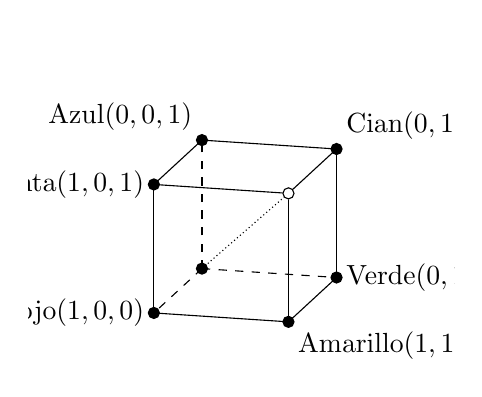
\begin{tikzpicture}
                \begin{axis}[view={105}{15},
                width=7cm,height=7cm,
                xtick=\empty,
                ytick=\empty,
                ztick=\empty,
                xmin=0, xmax=30,
                ymin=-10, ymax=30,
                zmin=-10, zmax=30,
                axis lines=center,
                axis line style={draw=none},
                ticks=none,
                ]
                    \def\radio{16}
                    \draw[dashed] (0,0,0) -- (\radio,0,0) node[left] {\makecell{Rojo \\ $(1, 0, 0)$}};
                    \draw[dashed] (0,0,0) -- (0,\radio,0) node[right] {\makecell{Verde \\ $(0, 1, 0)$}};
                    \draw[dashed] (0,0,0) -- (0,0,\radio) node[above left] {\makecell{Azul \\ $(0, 0, 1)$}};
                    \draw (\radio,0,0) -- (\radio,0,\radio) node[left] {\makecell{Magenta \\ $(1, 0, 1)$}};
                    \draw (\radio,0,0) -- (\radio,\radio,0) node[below right] {\makecell{Amarillo \\ $(1, 1, 0)$}};
                    \draw (\radio,\radio,0) -- (0,\radio,0);
                    \draw (0,\radio,0) -- (0,\radio,\radio) node[above right] {\makecell{Cian \\ $(0, 1, 1)$}};
                    \draw[densely dotted] (0,0,0) -- (\radio,\radio,\radio);
                    \draw (\radio,\radio,0) -- (\radio,\radio,\radio);
                    \draw (0,0,\radio) -- (\radio,0,\radio) -- (\radio,\radio,\radio) -- (0,\radio,\radio) -- cycle;
                    %
                    \filldraw (0,0,0) circle (2pt);
                    \filldraw (\radio,0,0) circle (2pt);
                    \filldraw (\radio,\radio,0) circle (2pt);
                    \filldraw (0,\radio,0) circle (2pt);
                    \filldraw (0,0,\radio) circle (2pt);
                    \filldraw (\radio,0,\radio) circle (2pt);
                    \filldraw (0,\radio,\radio) circle (2pt);
                    \filldraw[white] (\radio,\radio,\radio) circle (2pt);
                    \draw (\radio,\radio,\radio) circle (2pt);
                \end{axis}
            \end{tikzpicture}
            \captionsetup*[figure]{hypcap=false}%
            \captionof{figure}{Representación del espacio de color RGB como un cubo en $\RR[3]$}
            \label{fig:cuboRGB}
        \end{center}
    \end{tcolorbox}
\end{adjustwidth}

\newpage

\begin{examplebox}{}{POLILINEAL}
    Demostrar que los polinomios
    $$1, x, x^2, \dots, x^n$$
    forman un conjunto linealmente independiente en $P_n$.

    \tcblower
    \solucion Por conveniencia, denotemos los polinomios como
    $$\mathbb{p}_0 = 1, \mathbb{p}_1 = x, \mathbb{p}_2 = x^2, \dots, \mathbb{p}_n = x^n.$$
    Debemos demostrar que los únicos coeficientes que satisfacen la ecuación vectorial
    \begin{equation}
        a_0\mathbb{p}_0 + a_1\mathbb{p}_1 + a_2\mathbb{p}_2 + \cdots + a_n\mathbb{p}_n = \mathbb{0} \label{eq:vectorial}
    \end{equation}
    son
    $$a_0 = a_1 = a_2 = \cdots = a_n = 0.$$
    La ecuación \eqref{eq:vectorial} es equivalente a la afirmación de que
    \begin{equation}
        a_0 + a_1x + a_2x^2 + \cdots + a_nx^n = 0 \label{eq:polinomial}
    \end{equation}
    para todo $x \in (-\infty, \infty)$. Por lo tanto, debemos demostrar que esto es cierto si y solo si cada coeficiente en \eqref{eq:polinomial} es igual a cero. Para ver que esto es cierto, recordemos del álgebra que un polinomio no nulo de grado $n$ tiene como máximo $n$ raíces distintas. Así, si alguno de los coeficientes en \eqref{eq:polinomial} no es cero, el lado izquierdo sería un polinomio no nulo con un número infinito de raíces, lo cual es una contradicción. Por lo tanto, la ecuación \eqref{eq:vectorial} solo tiene la solución trivial.
\end{examplebox}

\section{Base y dimensión}

\begin{definicion}{}{}
    Decimos que un conjunto finito de vectores $\{ \mathbb{v}_1, \mathbb{v}_2, \dots, \mathbb{v}_n \}$ es una \emph{base} para un espacio vectorial $V$ si:
    \begin{enumerate}[label=\roman*), topsep=6pt, itemsep=0pt]
        \item $\{ \mathbb{v}_1, \mathbb{v}_2, \dots, \mathbb{v}_n \}$ es linealmente independiente,
        \item $\{ \mathbb{v}_1, \mathbb{v}_2, \dots, \mathbb{v}_n \}$ genera a $V$.
    \end{enumerate}
\end{definicion}

Si se considera una base como la descripción de un sistema de coordenadas para un espacio vectorial $V$ de dimensión finita, entonces la parte (i) de esta definición garantiza que no existe ninguna interrelación entre los vectores base, la parte (ii) garantiza que hay suficientes vectores base para proporcionar coordenadas a todos los vectores en $V$. A continuación, se presentan algunos ejemplos.

\begin{examplebox}{}{}
    Recordemos del ejemplo \ref{examplebox:vectores_unitarios_generaRn} que los vectores unitarios estándar en
    \begin{matrizn}
        \makecell{\includegraphics[page=3]{Externalizacion/C1/MatricesC1.pdf}}
    \end{matrizn}
    generan $\RR[n]$ y del ejemplo \ref{examplebox:vectores_unitarios_liRn}, que son linealmente independientes. Por lo tanto, forman una base para $\RR[n]$ que llamamos \emph{base natural}, \emph{base estándar} o \emph{base canónica} para $\RR[n]$. En particular,
    \begin{matrizn}
        \makecell{\includegraphics[page=4]{Externalizacion/C1/MatricesC1.pdf}}
    \end{matrizn}
    es la base estándar para $\RR[3]$.
\end{examplebox}

\newpage

\begin{examplebox}{}{}
    Demostrar que $\mathcalm{B} = \left\{1, x, x^2, \dots, x^n\right\}$ es una base para el espacio vectorial $P_n$ de polinomios de grado $n$ o menor, que llamamos la \emph{base estándar} de $P_n$.
    
    \tcblower
    \solucion Debemos demostrar que los polinomios en $\mathcalm{B}$ son linealmente independientes y generan $P_n$. Denotemos estos polinomios como
    $$\mathbb{p}_0 = 1, \mathbb{p}_1 = x, \mathbb{p}_2 = x^2, \dots, \mathbb{p}_n = x^n.$$
    Mostramos en el ejemplo \ref{examplebox:POLIGENERA} que estos vectores generan $P_n$ y en el ejemplo \ref{examplebox:POLILINEAL} que son linealmente independientes. Por lo tanto, forman una base para $P_n$.
\end{examplebox}

\begin{examplebox}{}{}
    Consideremos el espacio vectorial $\RR[3]$ y el conjunto
    \begin{matrizn}
        \makecell{\includegraphics[page=13]{Externalizacion/C1/MatricesC1.pdf}}
    \end{matrizn}
    Queremos demostrar que este conjunto es una base de $\RR[3]$. Para verificar que $\mathcalm{B}$ es linealmente independiente, formamos la ecuación
    \begin{matrizn}
        \makecell{\includegraphics[page=14]{Externalizacion/C1/MatricesC1.pdf}}
    \end{matrizn}
    y resolvemos para $c_1$, $c_2$, $c_3$. De lo anterior, obtenemos el siguiente sistema lineal
    \begin{align*}
        c_1 + c_3 & = 0 \\
        c_1 + c_2 & = 0 \\
        c_2 + c_3 & = 0
    \end{align*}
    que tiene como única solución $c_1 = c_2 = c_3 = c_4 = 0$, lo cual muestra que $\mathcalm{B}$ es linealmente independiente. Para mostrar que $\mathcalm{B}$ genera a $\RR[3]$, debemos probar que cualquier vector en $\RR[3]$ se puede expresar como combinación lineal de $\mathcalm{B}$, es decir, debemos encontrar constantes $c_1$, $c_2$, $c_3$ tales que
    \begin{matrizn}
        \makecell{\includegraphics[page=15]{Externalizacion/C1/MatricesC1.pdf}}
    \end{matrizn}
    De la expresión anterior, obtenemos el siguiente sistema lineal
    \begin{align*}
        c_1 + c_3 & = x \\
        c_1 + c_2 & = y \\
        c_2 + c_3 & = z
    \end{align*}
    que tiene como única solución
    $$c_1 = \frac{x + y - z}{2}, \quad c_2 = - \frac{x - y - z}{2}, \quad c_3 = \frac{x - y + z}{2}.$$
    Por lo tanto, $\mathcalm{B}$ genera a $\RR[3]$. Se concluye así que $\mathcalm{B}$ es una base para $\RR[3]$.
\end{examplebox}

\begin{examplebox}{}{}
    Determine una base para el subespacio de $P_2$, formado por los vectores de la forma $at^2 + bt + c$ donde $c = a - b$.

    \tcblower
    \solucion Todo vector en $V$ es de la forma
    $$at^2 + bt + a - b,$$
    que puede escribirse como
    $$a(t^2 + 1) + b(t - 1),$$
    \newpage
    lo cual muestra que los vectores $t^2 + 1$ y $t - 1$ generan a $V$. Además, estos vectores son linealmente independientes ya que ninguno es múltiplo del otro. También podría haberse obtenido (con mayor trabajo) esta conclusión sobre independencia lineal, escribiendo la ecuación
    $$a_1(t^2 + 1) + a_2(t - 1) = 0$$
    o
    $$t^2 a_1 + t a_2 + (a_1 - a_2) = 0.$$
    Como esta ecuación se cumple para todos los valores de $t$, debemos tener $a_1 = 0$ y $a_2 = 0$, que es la condición de independencia lineal.
\end{examplebox}

\begin{definicion}{}{}
    Sea $V$ un espacio vectorial sobre $K$. Se llama \emph{dimensión} del espacio vectorial $V$, a la cardinalidad de la base de $V$, y se denotará por $\Dim V$.
\end{definicion}

Un espacio vectorial es de \emph{dimensión finita} si existe un subconjunto finito de $V$ que es una base para $V$; en caso contrario, es decir, si no existe tal subconjunto finito, el espacio es de \emph{dimensión infinita}.

Casi todos los espacios vectoriales considerados en este libro son de dimensión finita. Sin embargo, es conveniente anotar que muchos espacios vectoriales de importancia en matemáticas y en física son de dimensión infinita; su estudio excede el alcance de este libro. El espacio vectorial $P$, de todos los polinomios, y el espacio vectorial $C(-\infty, \infty)$ de las funciones continuas $f: \RR \longrightarrow \RR$, no son de dimensión finita.

Ahora estableceremos algunos resultados relativos a espacios vectoriales de dimensión finita, que hacen referencia al número de vectores en una base, comparan el número de vectores de dos bases diferentes y establecen propiedades de las bases.

\begin{theorem}{}{}
    Sea $V$ un espacio vectorial y sea $\mathcalm{B} = \{ \mathbb{v}_1, \mathbb{v}_2, \dots, \mathbb{v}_n \}$ una base de $V$. Entonces todo elemento de $V$ se expresa de manera única a partir de los elementos de la base. Es decir, dado $\mathbb{u} \in V$, existen escalares $a_1$, $a_2$, $\dots$, $a_n$ únicos tales que
    \begin{equation}
        \mathbb{u} = a_1\mathbb{v}_1 + a_2\mathbb{v}_2 + \cdots + a_n\mathbb{v}_n \label{ec25}
    \end{equation}

    \tcblower
    \demostracion Supongamos que existen escalares $b_1$, $b_2$, $\dots$, $b_n$ tales que
    \begin{equation}
        \mathbb{u} = b_1\mathbb{v}_1 + b_2\mathbb{v}_2 + \cdots + b_n\mathbb{v}_n \label{ec26}
    \end{equation}
    Se demostrará que $a_i = b_i$, para $i = 1$, $2$, $\dots$, $n$. Sea
    \begin{align*}
        -\mathbb{u} & = (-1) \cdot \mathbb{u} \\
        & = (-1) \cdot (b_1\mathbb{v}_1 + b_2\mathbb{v}_2 + \cdots + b_n\mathbb{v}_n) \\
        & = (-1)b_1\mathbb{v}_1 + (-1)b_2\mathbb{v}_2 + \cdots + (-1)b_n\mathbb{v}_n \\
        & = (-b_1)\mathbb{v}_1 + (-b_2)\mathbb{v}_2 + \cdots + (-b_n)\mathbb{v}_n
    \end{align*}
    Ahora, de las expresiones \eqref{ec25} y \eqref{ec26} tenemos
    \begin{align*}
        \mathbb{0} & = \mathbb{u} + (-\mathbb{u}) \\
        & = a_1\mathbb{v}_1 + a_2\mathbb{v}_2 + \cdots + a_n\mathbb{v}_n + (-b_1)\mathbb{v}_1 + (-b_2)\mathbb{v}_2 + \cdots + (-b_n)\mathbb{v}_n \\
        & = \big(a_1+(-b_1)\big)\mathbb{v}_1 + \big(a_2+(-b_2)\big)\mathbb{v}_2 + \cdots + \big(a_n+(-b_n)\big)\mathbb{v}_n
    \end{align*}
    Como $\mathcalm{B}$ es linealmente independiente,
    $$\big(a_1+(-b_1)\big) = 0, \big(a_2+(-b_2)\big) = 0, \dots, \big(a_n+(-b_n)\big) = 0,$$
    de modo que $b_1 = a_1$, $b_2 = a_2$, $\dots$, $b_n = a_n$. Por lo tanto, solo hay una forma de expresar $\mathbb{u}$ como combinación lineal de los vectores en $\mathcalm{B}$.
\end{theorem}

\newpage

Supongamos que $\mathcalm{B} = \{\mathbb{v}_1, \mathbb{v}_2, \dots, \mathbb{v}_n\}$ genera un espacio vectorial $V$ y que $\mathbb{v}_j$ es una combinación lineal de los vectores que le preceden en $\mathcalm{B}$. Entonces el conjunto
$$\mathcalm{A} = \{\mathbb{v}_1, \mathbb{v}_2, \dots, \mathbb{v}_{j-1}, \mathbb{v}_{j+1}, \dots, \mathbb{v}_n\}$$
que consta de los vectores en $\mathcalm{B}$, con excepción de $\mathbb{v}_j$, también genera a $V$. Para demostrar este resultado, observemos que si $\mathbb{v}$ es cualquier vector en $V$, entonces, como $\mathcalm{B}$ genera a $V$, podemos encontrar escalares $a_1$, $a_2$, $\dots$, $a_n$ tales que
$$\mathbb{v} = a_1 \mathbb{v}_1 + a_2 \mathbb{v}_2 + \cdots + a_{j-1} \mathbb{v}_{j-1} + a_j \mathbb{v}_j + a_{j+1} \mathbb{v}_{j+1} + \cdots + a_n \mathbb{v}_n.$$
Ahora, si
$$\mathbb{v}_j = b_1 \mathbb{v}_1 + b_2 \mathbb{v}_2 + \cdots + b_{j-1} \mathbb{v}_{j-1},$$
entonces
\begin{align*}
    \mathbb{v} & = a_1 \mathbb{v}_1 + a_2 \mathbb{v}_2 + \cdots + a_{j-1} \mathbb{v}_{j-1} + a_j (b_1 \mathbb{v}_1 + b_2 \mathbb{v}_2 + \cdots + b_{j-1} \mathbb{v}_{j-1}) \\
    & \hspace{3cm} + a_{j+1} \mathbb{v}_{j+1} + \cdots + a_n \mathbb{v}_n \\
    & = c_1 \mathbb{v}_1 + c_2 \mathbb{v}_2 + \cdots + c_{j-1} \mathbb{v}_{j-1} + c_{j+1} \mathbb{v}_{j+1} + \cdots + c_n \mathbb{v}_n
\end{align*}
lo cual significa que $\Gen \mathcalm{A} = V$.

\begin{theorem}{}{algunsubbW}
    Sea $\mathcalm{B} = \{\mathbb{v}_1, \mathbb{v}_2, \dots, \mathbb{v}_n\}$ un conjunto de vectores no nulos en un espacio vectorial $V$ y sea $W = \Gen \mathcalm{B}$. Entonces, algún subconjunto de $\mathcalm{B}$ es una base para $W$.

    \tcblower
    \demostracion Procedamos por casos.
    \begin{enumerate}[label=\roman*), topsep=6pt, itemsep=0pt]
        \item Si $\mathcalm{B}$ es linealmente independiente, entonces $\mathcalm{B}$ es una base para $W$ porque $\mathcalm{B}$ es generador de $W$, de acuerdo con la hipótesis.
        \item Si $\mathcalm{B}$ es linealmente dependiente, entonces existen $c_1, c_2, \dots, c_n$, no todos iguales a cero, tales que
        $$c_1 \mathbb{v}_1 + c_2 \mathbb{v}_2 + \cdots + c_n \mathbb{v}_n = \mathbb{0}.$$
        Por lo tanto, algún $\mathbb{v}_j$ es una combinación lineal de los vectores anteriores en $\mathcalm{B}$ (teorema \ref{theorem:licombinacion_lineal}). Ahora, eliminamos $\mathbb{v}_j$ de $\mathcalm{B}$, para obtener un subconjunto $\mathcalm{B}_1$ de $\mathcalm{B}$. Entonces, por la observación anterior a este teorema, concluimos que $\mathcalm{B}_1 = \{\mathbb{v}_1, \mathbb{v}_2, \dots, \mathbb{v}_{j-1}, \mathbb{v}_{j+1}, \dots, \mathbb{v}_n\}$ genera a $W$. Si $\mathcalm{B}_1$ es linealmente independiente, entonces $\mathcalm{B}_1$ es una base. Si $\mathcalm{B}_1$ es linealmente dependiente, eliminamos un vector de $\mathcalm{B}_1$ que sea combinación lineal de los vectores que le preceden en $\mathcalm{B}_1$ y obtenemos un nuevo conjunto $\mathcalm{B}_2$ que también genera a $W$. Continuando de esta forma, y dado que $\mathcalm{B}$ es un conjunto finito, en algún momento encontraremos un subconjunto $\mathcalm{A}$ de $\mathcalm{B}$ que es linealmente independiente y genera a $W$. Tal conjunto $\mathcalm{A}$ es una base para $W$.
    \end{enumerate}
\end{theorem}

\begin{examplebox}{}{}
    La dimensión de $\RR[2]$ es $2$; la dimensión de $\RR[3]$ es $3$; y en general, la dimensión de $\RR[n]$ es $n$. Esto se expresa respectivamente como $\Dim \RR[2] = 2$, $\Dim \RR[3] = 3$, $\Dim \RR[n] = n$.
\end{examplebox}

\begin{examplebox}{}{}
    La dimensión de $P_2$ es $3$; la dimensión de $P_3$ es $4$; y en general, la dimensión de $P_n$ es $n + 1$. Esto se expresa respectivamente como $\Dim P_2 = 3$, $\Dim P_3 = 4$, $\Dim P_n = n + 1$.
\end{examplebox}

\begin{examplebox}{}{}
    Si $\mathcalm{B} = \{\mathbb{v}_1, \mathbb{v}_2, \dots, \mathbb{v}_r\}$, entonces cada vector en $\Gen \mathcalm{B}$ se puede expresar como una combinación lineal de los vectores en $\mathcalm{B}$. Así, si los vectores en $\mathcalm{B}$ son linealmente independientes, automáticamente forman una base para $\Gen \mathcalm{B}$, de lo cual podemos concluir que
    $$\Dim \Gen(\{\mathbb{v}_1, \mathbb{v}_2, \dots, \mathbb{v}_r\}) = r.$$
    En otras palabras, la dimensión del espacio generado por un conjunto linealmente independiente de vectores es igual al número de vectores en ese conjunto.
\end{examplebox}

\newpage

Observemos que si $\{ \mathbb{v}_1, \mathbb{v}_2, \dots, \mathbb{v}_n \}$ es una base para un espacio vectorial $V$, entonces $\{ c\mathbb{v}_1, c\mathbb{v}_2, \dots, c\mathbb{v}_n \}$ también es una base, si $c \neq 0$. Esta observación muestra que un espacio vectorial real diferente de $\mathbb{0}$ tiene siempre infinitas bases.

\begin{theorem}{}{vmenorli}
    Sea $V$ un espacio vectorial de dimensión finita. Si $\mathcalm{B} = \{\mathbb{v}_1, \mathbb{v}_2, \dots, \mathbb{v}_n\}$ es una base para $V$ y $\mathcalm{A} = \{\mathbb{w}_1, \mathbb{w}_2, \dots, \mathbb{w}_r\}$ es un conjunto linealmente independiente de vectores en $V$, entonces $r \leq n$.

    \tcblower
    \demostracion Sea $\mathcalm{A}_1 = \{\mathbb{w}_1, \mathbb{v}_1, \mathbb{v}_2, \dots, \mathbb{v}_n\}$. Como $\mathcalm{B}$ genera a $V$, $\mathcalm{A}_1$ también lo genera. Y, puesto que $\mathbb{w}_1$ es una combinación lineal de los vectores de $\mathcalm{B}$, $\mathcalm{A}_1$ es linealmente dependiente. Entonces, de acuerdo con el teorema \ref{theorem:licombinacion_lineal}, algún $\mathbb{v}_j$ es una combinación lineal de los vectores que le preceden en $\mathcalm{A}_1$. Eliminemos ese vector particular $\mathbb{v}_j$. Sea $\mathcalm{B}_1 = \{\mathbb{w}_1, \mathbb{v}_1, \dots, \mathbb{v}_{j-1}, \mathbb{v}_{j+1}, \dots, \mathbb{v}_n\}$. Observemos que $\mathcalm{B}_1$ genera a $V$. A continuación, sea $\mathcalm{A}_2 = \{\mathbb{w}_2, \mathbb{w}_1, \mathbb{v}_1, \dots, \mathbb{v}_{j-1}, \mathbb{v}_{j+1}, \dots, \mathbb{v}_n\}$. Entonces $\mathcalm{A}_2$ es linealmente dependiente, y algún vector en $\mathcalm{A}_2$ es una combinación lineal de los vectores precedentes en $\mathcalm{A}_2$. Como $\mathcalm{A}$ es linealmente independiente, dicho vector no puede ser $\mathbb{w}_1$, así que es $\mathbb{v}_i$, con $i \neq j$. Repetimos este proceso una y otra vez. Si se eliminan todos los vectores $\mathbb{v}$ antes de que se puedan incluir todos los vectores $\mathbb{w}$, entonces el conjunto resultante de vectores $\mathbb{w}$, un subconjunto de $\mathcalm{A}$, es linealmente dependiente, lo cual implica que también $\mathcalm{A}$ es linealmente dependiente. Esta contradicción permite concluir que el número $r$ de vectores $\mathbb{w}$ no puede ser mayor que el número $n$ de vectores $\mathbb{v}$. Esto es, $r \leq n$.
\end{theorem}

\begin{corollary}{}{}
    Si $\mathcalm{B} = \{\mathbb{v}_1, \mathbb{v}_2, \dots, \mathbb{v}_n\}$ y $\mathcalm{A} = \{\mathbb{w}_1, \mathbb{w}_2, \dots, \mathbb{w}_m\}$ son dos bases para un espacio vectorial, entonces $n = m$.

    \tcblower
    \demostracion Como $\mathcalm{A}$ es un conjunto linealmente independiente de vectores, el teorema \ref{theorem:vmenorli} implica que $m \leq n$. Igualmente, tenemos que $n \leq m$, puesto que $\mathcalm{B}$ es linealmente independiente. Entonces, $n = m$.
\end{corollary}

Se puede probar que todos los espacios de dimensión finita que tienen igual dimensión difieren solo en la naturaleza de sus elementos; sus propiedades algebraicas son idénticas.

A continuación, enunciaremos una consecuencia directa del teorema \ref{theorem:vmenorli}.

\begin{theorem}{}{}
    Sea $V$ un espacio vectorial de dimensión finita $n$, y sea $W$ un subespacio no nulo de $V$, entonces $\Dim W \leq \Dim V$.

    \tcblower
    \demostracion Sea $\{ \mathbb{v}_1, \mathbb{v}_2, \dots, \mathbb{v}_k \}$ una base de $W$. Al ser una base, los vectores $\mathbb{v}_1, \mathbb{v}_2, \dots, \mathbb{v}_k$ son linealmente independientes. Por el teorema \ref{theorem:vmenorli}, sabemos que $k \leq n$, de donde se sigue que
    $$\Dim W = k \leq n = \Dim V.$$
    Por lo tanto, $\Dim W \leq \Dim V$.
\end{theorem}

En la observación anterior al teorema \ref{theorem:vmenorli} mencionamos que un espacio vectorial tiene muchas bases; pero acabamos de demostrar que, para un espacio vectorial particular $V$, todas las bases tienen el mismo número de vectores. Este hecho conduce a la propia definición de dimensión.

Se puede probar que si un espacio vectorial $V$ tiene dimensión finita $n$, entonces cualquier conjunto de $n + 1$ vectores en $V$ es linealmente dependiente. En particular, cualquier conjunto con más de $n$ vectores en $\RR[n]$ es linealmente dependiente (teorema \ref{theorem:Rnldsinmm}. A continuación, demostraremos que si $\Dim V = n$, entonces ningún conjunto de $n - 1$ vectores en $V$ puede generar a $V$. Por ejemplo, sabemos que la dimensión de $P_2$ es $3$. Entonces el conjunto $\left\{ 1 - x^2, x \right\}$ no puede ser una base de $P_2$, pues tendríamos a lo más dos vectores linealmente independientes y $2 < 3 = \Dim P_2$.

\newpage

\begin{theorem}{}{}
    Si $V$ es un espacio vectorial de dimensión finita $n$, entonces ningún conjunto con $n - 1$ vectores de $V$ puede generar a $V$.

    \tcblower
    \demostracion Sea $V$ un espacio vectorial de dimensión finita $n$. Supongamos que $\mathcalm{B} = \{\mathbb{v}_1, \mathbb{v}_2, \dots, \mathbb{v}_{n-1}\}$ es subconjunto de $V$ y que además, $\mathcalm{B}$ genera $V$. Entonces, por el teorema \ref{theorem:algunsubbW} existe un subconjunto $\mathcalm{B}_1$ de $\mathcalm{B}$ tal que $\mathcalm{B}_1$ es una base de $V$. Dado que $\mathcalm{B}_1$ es una base de $V$, tenemos que
    \begin{equation}
        \Dim V = |\mathcalm{B}_1|. \label{IAOQPOQIQI}
    \end{equation}
    Como $\mathcalm{B}_1$ es subconjunto de $\mathcalm{B}$, se cumple que
    \begin{equation}
        |\mathcalm{B}_1| \leq |\mathcalm{B}| = n - 1. \label{AOPAPOBCCA}
    \end{equation}
    Las ecuaciones \eqref{IAOQPOQIQI} y \eqref{AOPAPOBCCA} juntas implican que
    $$\Dim V \leq n - 1 $$
    lo cual es una contradicción con la hipótesis de que $\Dim V = n$. Por lo tanto, $\mathcalm{B}$ no puede generar $V$.
\end{theorem}

De acuerdo con la definición, un conjunto de vectores en un espacio vectorial $V$ es una base para $V$ si genera a $V$ y es linealmente independiente. Sin embargo, si sabemos que la dimensión de $V$ es $n$, y el conjunto tiene $n$ vectores, solo necesitamos verificar una de las dos condiciones, de acuerdo con el siguiente teorema.

\begin{theorem}{}{siLIByGB}
    Sea $V$ un espacio vectorial de dimensión $n$ y sea $\mathcalm{B} = \{\mathbb{v}_1, \mathbb{v}_2, \dots, \mathbb{v}_n\}$ un conjunto de $n$ vectores en $V$.
    \begin{enumerate}[label=\roman*), topsep=6pt, itemsep=0pt]
        \item Si $\mathcalm{B}$ es linealmente independiente, entonces es una base para $V$.
        \item Si $\mathcalm{B}$ genera a $V$, entonces es una base para $V$.
    \end{enumerate}

    \tcblower
    \demostracion
    \begin{enumerate}[label=\roman*), topsep=6pt, itemsep=0pt]
        \item Dado que $\mathcalm{B}$ es linealmente independiente y $\dim V = n$, entonces existe una base $\mathcalm{A}$ para $V$, que contiene a $\mathcalm{B}$. Pero, dado que $\dim V = n$, $\mathcalm{A}$ no puede contener más elementos que $\mathcalm{B}$. Esto implica que $\mathcalm{B} = \mathcalm{A}$. Por lo tanto, $\mathcalm{B}$ es una base de $V$.
        \item Dado que $\mathcalm{B}$ genera $V$, podemos decir que algún subconjunto de $\mathcalm{B}$, digamos $\mathcalm{A}$, es una base de $V$. Como $\dim V = n$, el conjunto $\mathcalm{A}$ contiene exactamente $n$ elementos. Esto implica que $\mathcalm{B} = \mathcalm{A}$. Por lo tanto, $\mathcalm{B}$ es una base de $V$.
    \end{enumerate}
\end{theorem}

A continuación enunciaremos un teorema para construir una base que contenga un conjunto dado de vectores linealmente independientes.

\begin{theorem}{}{}
    Si $\mathcalm{A}$ es un conjunto de vectores linealmente independientes en un espacio vectorial de dimensión finita $V$, existe una base $\mathcalm{B}$ para $V$, que contiene a $\mathcalm{A}$.

    \tcblower
    \demostracion Sea $\mathcalm{A} = \{ \mathbb{v}_1, \mathbb{v}_2, \dots, \mathbb{v}_k \}$ un conjunto de vectores linealmente independientes en $V$, donde $k \leq n$. Como $V$ es de dimensión finita $n$, sabemos que existe una base $\mathcalm{B} = \{ \mathbb{v}_1, \mathbb{v}_2, \dots, \mathbb{v}_k, \mathbb{w}_1, \mathbb{w}_2, \dots, \mathbb{w}_{n-k} \}$ de $V$, donde los $\mathbb{w}_i$ son vectores adicionales que completan la base. Entonces, el conjunto $\mathcalm{B}$ genera a $V$. Ahora bien, queremos demostrar que $\mathcalm{A} \cup \{\mathbb{w}_1, \mathbb{w}_2, \dots, \mathbb{w}_{n-k}\}$ es un conjunto de vectores linealmente independientes. Es decir, debemos demostrar que
    $$c_1 \mathbb{v}_1 + c_2 \mathbb{v}_2 + \dots + c_k \mathbb{v}_k + d_1 \mathbb{w}_1 + d_2 \mathbb{w}_2 + \dots + d_{n-k} \mathbb{w}_{n-k} = 0.$$
    tiene como solución la trivial. Pero, $\mathcalm{A}$ es linealmente independiente, por lo que
    $$c_1 = c_2 = \dots = c_k = 0.$$
    \newpage
    Por lo tanto, la ecuación se reduce a
    $$d_1 \mathbb{w}_1 + d_2 \mathbb{w}_2 + \dots + d_{n-k} \mathbb{w}_{n-k} = 0.$$
    Como $\{ \mathbb{w}_1, \mathbb{w}_2, \dots, \mathbb{w}_{n-k} \}$ son parte de la base de $V$, también son linealmente independientes, lo que implica que
    $$d_1 = d_2 = \dots = d_{n-k} = 0.$$
	Esto demuestra que el conjunto $\{ \mathbb{v}_1, \mathbb{v}_2, \dots, \mathbb{v}_k, \mathbb{w}_1, \mathbb{w}_2, \dots, \mathbb{w}_{n-k} \}$ es linealmente independiente. Como el conjunto $\mathcalm{A} \cup \{ \mathbb{w}_1, \mathbb{w}_2, \dots, \mathbb{w}_{n-k} \}$ es linealmente independiente y tiene $n$ vectores, entonces este conjunto es una base de $V$.
\end{theorem}

El teorema anterior establece que un conjunto linealmente independiente de vectores en un espacio vectorial $V$ puede extenderse a una base para $V$.

\begin{examplebox}{}{}
    Sea $V = \RR[3]$ y sea el conjunto de vectores $\mathcalm{A} = \{ \mathbb{v}_1, \mathbb{v}_2 \}$, donde
    \begin{matrizn}
        \makecell{\includegraphics[page=16]{Externalizacion/C1/MatricesC1.pdf}}
    \end{matrizn}
    Queremos demostrar que existe una base $\mathcalm{B}$ para $V$ que contenga a $\mathcalm{A}$. Notemos que $\mathcalm{A}$ es linealmente independiente, ya que no existe un escalar $c$ tal que $c\mathbb{v}_1 = \mathbb{v}_2$. Aunque $\mathcalm{A}$ es linealmente independiente en $\RR[3]$, no contiene tres vectores. Como $\RR[3]$ tiene dimensión 3, necesitamos agregar un tercer vector a $\mathcalm{A}$ para completar la base de $V$. Podemos elegir un tercer vector, por ejemplo,
    \begin{matrizn}
        \makecell{\includegraphics[page=17]{Externalizacion/C1/MatricesC1.pdf}}
    \end{matrizn}
    que no es combinación lineal de los vectores en $\mathcalm{A}$. Ahora, debemos verificar que
    $$\mathcalm{B} = \{ \mathbb{v}_1, \mathbb{v}_2, \mathbb{v}_3 \}$$
    es linealmente independiente, pero este es linealmente independiente ya que ninguno de estos vectores puede escribirse como una combinación lineal de los otros. Además, $\mathcalm{B}$ genera $\RR[3]$, porque cualquier vector en $\RR[3]$ puede escribirse como una combinación lineal de estos tres vectores. Es decir,
    \begin{matrizn}
        \makecell{\includegraphics[page=18]{Externalizacion/C1/MatricesC1.pdf}}
    \end{matrizn}
    cuya solución es
    $$c_1 = y, \quad c_2 = x - y, \quad c_3 = -x + y + z.$$
    Por lo tanto, $\mathcalm{B}$ es una base para $\RR[3]$ y contiene al conjunto $\mathcalm{A}$.
\end{examplebox}

Recordemos que la dimensión de un espacio vectorial se define como la cantidad de vectores linealmente independientes necesarios para generar todo el espacio. En el caso del vector cero, su dimensión es $0$ porque no puede generar ningún otro vector aparte de sí mismo mediante combinaciones lineales. Para entenderlo mejor, consideremos que cualquier vector $\mathbb{v}$ en un espacio vectorial $V$ puede ser expresado como
$$\mathbb{v} = c_1 \mathbb{v}_1 + c_2 \mathbb{v}_2 + \cdots + c_n \mathbb{v}_n$$
donde $\mathbb{v}_1, \mathbb{v}_2, \dots, \mathbb{v}_n$ son vectores linealmente independientes en $V$, y $c_1, c_2, \dots, c_n$ son escalares. Ahora, si consideramos el vector cero, no importa cuánto intentemos expresarlo como una combinación lineal de otros vectores $\mathbb{v}_1, \mathbb{v}_2, \dots, \mathbb{v}_n$, siempre obtendremos $\mathbb{0}$ como resultado, ya que cualquier escalar multiplicado por $\mathbb{0}$ sigue siendo $\mathbb{0}$.

\newpage

\begin{theorem}{}{dimSumadeSEV}
    Sea $V$ un espacio vectorial de dimensión finita $n$. Si $S$ y $T$ son subespacios de $V$, entonces
    $$\Dim (S + T) = \Dim(S) + \Dim(T) - \Dim(S \cap T).$$

    \tcblower
    \demostracion Como $S$ y $T$ son subespacios de $V$, entonces $S + T$ y $S \cap T$ son subespacios de $V$ (por el ejercicio \ref{ejercicio_sumadesubs}, pág. \pageref{ejercicio_sumadesubs} y teorema \ref{theorem:intersubsV}). Además, como $V$ es de dimensión finita, entonces $S$, $T$, $S + T$ y $S \cap T$ son de dimensión finita. Sean
    $$\dim S = r, \quad \dim T = m, \quad \dim (S \cap T) = k.$$
    Sea
    $$\{\mathbb{u}_1, \mathbb{u}_2, \dots, \mathbb{u}_k\}$$
    una base de $S \cap T$. Claro que $\{\mathbb{u}_1, \mathbb{u}_2, \dots, \mathbb{u}_k\} \subset S$ es linealmente independiente y podemos completarlo con $\mathbb{v}_1, \mathbb{v}_2, \dots, \mathbb{v}_{r-k} \in S$ a una base de $S$, y por tanto
    $$\{\mathbb{u}_1, \mathbb{u}_2, \dots, \mathbb{u}_k, \mathbb{v}_1, \mathbb{v}_2, \dots, \mathbb{v}_{r-k}\}$$
    es una base de $S$. Análogamente, $\{\mathbb{u}_1, \mathbb{u}_2, \dots, \mathbb{u}_k\} \subset T$ es linealmente independiente y podemos completarlo con $\mathbb{w}_1, \mathbb{w}_2, \dots, \mathbb{w}_{m-k} \in T$ a una base de $T$, y por tanto
    $$\{\mathbb{u}_1, \mathbb{u}_2, \dots, \mathbb{u}_k, \mathbb{w}_1, \mathbb{w}_2, \dots, \mathbb{w}_{m-k}\}$$
    es una base de $T$. Probaremos enseguida que
    $$\mathcalm{B} = \{\mathbb{v}_1, \mathbb{v}_2, \dots, \mathbb{v}_{r-k}, \mathbb{u}_1, \mathbb{u}_2, \dots, \mathbb{u}_k, \mathbb{w}_1, \mathbb{w}_2, \dots, \mathbb{w}_{m-k}\}$$
    es una base de $S + T$. Primero, demostremos que, en efecto, $\mathcalm{B}$ genera a $S + T$. Sea $\mathbb{s} \in S + T$, entonces $\mathbb{s} = \mathbb{u} + \mathbb{v}$. Es decir, existen $s_1, \dots, s_k, b_1, \dots, b_{r-k}$ y $t_1, \dots, t_k, a_1, \dots, a_{m-k}$ escalares tales que
    $$\mathbb{u} = s_1 \mathbb{u}_1 + \cdots + s_k \mathbb{u}_k + b_1 \mathbb{v}_1 + \cdots + b_{r-k} \mathbb{v}_{r-k}$$
    y
    $$\mathbb{v} = t_1 \mathbb{u}_1 + \cdots + t_k \mathbb{u}_k + a_1 \mathbb{w}_1 + \cdots + a_{m-k} \mathbb{w}_{m-k}.$$
    Lo que nos lleva a que
    $$\mathbb{s} = b_1 \mathbb{v}_1 + \cdots + b_{r-k} \mathbb{v}_{r-k} + (s_1 + t_1)\mathbb{u}_1 + \cdots + (s_k + t_k)\mathbb{u}_k + a_1 \mathbb{w}_1 + \cdots + a_{m-k} \mathbb{w}_{m-k}.$$
    Por lo tanto, $\mathbb{s} \in \Gen (\{\mathbb{v}_1, \dots, \mathbb{v}_{r-k}, \mathbb{u}_1, \dots, \mathbb{u}_k, \mathbb{w}_1, \dots, \mathbb{w}_{m-k}\})$, lo que implica que $\mathcalm{B}$ genera a $S + T$. Ahora, demostremos que, en efecto, $\mathcalm{B}$ es linealmente independiente. Sean $x_1, \dots, x_{r-k}, y_1, \dots, y_k, z_1, \dots, z_{m-k}$ escalares tales que
    $$0 = x_1 \mathbb{v}_1 + \dots + x_{r-k} \mathbb{v}_{r-k} + y_1 \mathbb{u}_1 + \dots + y_k \mathbb{u}_k + z_1 \mathbb{w}_1 + \dots + z_{m-k} \mathbb{w}_{m-k}.$$
    Entonces
    $$x_1 \mathbb{v}_1 + \dots + x_{r-k} \mathbb{v}_{r-k} = -(y_1 \mathbb{u}_1 + \dots + y_k \mathbb{u}_k + z_1 \mathbb{w}_1 + \dots + z_{m-k} \mathbb{w}_{m-k}),$$
    por tanto
    $$x_1 \mathbb{v}_1 + \dots + x_{r-k} \mathbb{v}_{r-k} \in T.$$
    Como
    $$x_1 \mathbb{v}_1 + \dots + x_{r-k} \mathbb{v}_{r-k} \in S,$$
    entonces
    $$x_1 \mathbb{v}_1 + \dots + x_{r-k} \mathbb{v}_{r-k} \in S \cap T.$$
    Por tanto existen $c_1, \dots, c_k$ escalares tales que
    $$x_1 \mathbb{v}_1 + \dots + x_{r-k} \mathbb{v}_{r-k} = c_1 \mathbb{u}_1 + \dots + c_k \mathbb{u}_k.$$
    Consecuentemente
    $$y_1 \mathbb{u}_1 + \dots + y_k \mathbb{u}_k + z_1 \mathbb{w}_1 + \dots + z_{m-k} \mathbb{w}_{m-k} = 0,$$
    \newpage
    y como
    $$\{\mathbb{u}_1, \mathbb{u}_2, \dots, \mathbb{u}_k, \mathbb{w}_1, \mathbb{w}_2, \dots, \mathbb{w}_{m-k}\}$$
    es base de $T$, entonces
    $$0 = y_1 = \dots = y_k = z_1 = \dots = z_{m-k}.$$
    Por tanto
    $$\{\mathbb{v}_1, \mathbb{v}_2, \dots, \mathbb{v}_{r-k}, \mathbb{u}_1, \mathbb{u}_2, \dots, \mathbb{u}_k, \mathbb{w}_1, \mathbb{w}_2, \dots, \mathbb{w}_{m-k}\}$$
    es linealmente independiente. Por todo lo anterior,
    $$\{\mathbb{v}_1, \mathbb{v}_2, \dots, \mathbb{v}_{r-k}, \mathbb{u}_1, \mathbb{u}_2, \dots, \mathbb{u}_k, \mathbb{w}_1, \mathbb{w}_2, \dots, \mathbb{w}_{m-k}\}$$
    es base de $S + T$, entonces
    \begin{align*}
        \dim(S + T) & = (r - k) + k + (m - k) \\
        & = r + m - k \\
        & = \dim S + \dim T - \dim(S \cap T)
    \end{align*}
\end{theorem}

\begin{examplebox}{}{}
    En $P_3$, sean
    $$W_1 = \left\{ p(x) \in P_3 \text{ tal que } x^2 - 1 \mid p(x) \right\}$$
    y
    $$W_2 = \left\{ p(x) \in P_3 \text{ tal que } x^2 + x - 2 \mid p(x) \right\}.$$
    Obtenga una base y la dimensión de los siguientes subespacios:
    \begin{tasks}(4)
        \task $W_1$,
        \task $W_2$,
        \task $W_1 \cap W_2$,
        \task $W_1 + W_2$.
    \end{tasks}

    \tcblower
    \demostracion Antes de empezar, recordemos la definición de divisibilidad de polinomios: Sean $f(x)$, $g(x) \in P_n$. Decimos que $g(x)$ divide a $f(x)$, o que $g(x)$ es un factor de $f(x)$, si existe $q(x) \in P_n$ tal que $f(x) = g(x)q(x)$. Comúnmente, para decir que $g(x)$ divide a $f(x)$ se escribe $g(x) \mid f(x)$.
    \begin{enumerate}[label=\alph*), topsep=6pt, itemsep=0pt]
        \item Sea $p(x) \in P_3$, con $p(x) = a_0 + a_1x + a_2x^2 + a_3x^3$, entonces
        \begin{align*}
            p(x) \in W_1 & \Longleftrightarrow x^2 - 1 \mid p(x) \\
            & \Longleftrightarrow \exists q(x) \in P_3 \text{ tal que } p(x) = \left( x^2 - 1 \right) q(x) \\
            & \Longleftrightarrow p(x) = \left( x^2 - 1 \right) (ax + b) \\
            & \Longleftrightarrow p(x) = a\left( x^3 - x \right) + b\left( x^2 - 1 \right)
        \end{align*}
        Por lo tanto, $p(x) \in \Gen \left(\left\{ x^3 - x, x^2 - 1 \right\}\right)$, y como no existe un escalar $c$ tal que $x^2 - 1 = c \left( x^3 - x \right)$, entonces el conjunto $\left\{ x^3 - x, x^2 - 1 \right\}$ es linealmente independiente. Además, es claro que dicho conjunto genera a $W_1$, pues para cualquier escalar $a$ y $b$, $p(x) \in W_1$. Por lo tanto, demostramos que $\mathcalm{A} = \left\{ x^3 - x, x^2 - 1 \right\}$ es una base para $W_1$ y por consiguiente, tenemos que $\Dim W_1 = 2$.
        \item Sea $p(x) \in P_3$, con $p(x) = a_0 + a_1x + a_2x^2 + a_3x^3$, entonces
        \begin{align*}
            p(x) \in W_2 & \Longleftrightarrow x^2 + x - 2 \mid p(x) \\
            & \Longleftrightarrow \exists q(x) \in P_3 \text{ tal que } p(x) = \left( x^2 + x - 2 \right) q(x) \\
            & \Longleftrightarrow p(x) = \left( x^2 + x - 2 \right) (ax + b) \\
            & \Longleftrightarrow p(x) = a\left( x^3 + x^2 - 2x \right) + b\left( x^2 + x - 2 \right)
        \end{align*}
        Por lo tanto, $p(x) \in \Gen \left(\left\{ x^3 + x^2 - 2x, x^2 + x - 2 \right\}\right)$, y como no existe un escalar $c$ tal que $x^3 + x^2 - 2x = c \left( x^2 + x - 2 \right)$, entonces el conjunto $\left\{ x^3 + x^2 - 2x, x^2 + x - 2 \right\}$ es linealmente independiente. Además, es claro que dicho conjunto genera a $W_2$, pues para cualquier $a$ y $b$, $p(x) \in W_2$. Por lo tanto, demostramos que $\mathcalm{B} = \left\{ x^3 + x^2 - 2x, x^2 + x - 2 \right\}$ es una base para $W_2$ y por consiguiente, tenemos que $\Dim W_2 = 2$.
        \item Sea $p(x) \in P_3$, con $p(x) = a_0 + a_1x + a_2x^2 + a_3x^3$, entonces
        \begin{align*}
            p(x) \in W_1 \cap W_2 & \Longleftrightarrow x^2 - 1 \mid p(x) \text{ y } x^2 + x - 2 \mid p(x) \\
            & \Longleftrightarrow (x - 1)(x + 1) \mid p(x) \text{ y } (x - 1)(x + 2) \mid p(x) \\
            & \Longleftrightarrow (x - 1)(x + 1)(x + 2) \mid p(x) \\
            & \Longleftrightarrow c \left( x^3 + 2x^2 - x - 2 \right)
        \end{align*}
        Por lo tanto, $p(x) \in \Gen \left(\left\{ x^3 + 2x^2 - x - 2 \right\}\right)$, y es linealmente independiente, pues es un conjunto de un solo elemento. Además, es claro que dicho conjunto genera a $W_1 \cap W_2$, pues para cualquier escalar $c$, $p(x) \in W_1 \cap W_2$. Por lo tanto, demostramos que $\mathcalm{C} = \left\{ x^3 + 2x^2 - x - 2 \right\}$ es una base de $W_1 \cap W_2$ y por consiguiente, $\Dim (W_1 \cap W_2) = 1$.
        \item Por el ejercicio \ref{ejercicio_sumadesubs} en la página \pageref{ejercicio_sumadesubs}, tenemos que
        \begin{align*}
            W_1 + W_2 & = \Gen(\mathcalm{A} \cup \mathcalm{B}) \\
            & = \Gen \left(\left\{ x^3 - x, x^2 - 1, x^3 + x^2 - 2x, x^2 + x - 2 \right\}\right)
        \end{align*}
        Observemos que
        $$x^2 + x - 2 = \left( x^3 - x \right) + 2\left( x^2 - 1 \right) - \left( x^3 + x^2 - 2x \right).$$
        Por lo tanto, $x^2 + x - 2$ es linealmente dependiente de los otros polinomios y se elimina. Los polinomios restantes forman el conjunto
        $$\mathcalm{D} = \left\{ x^3 - x, x^2 - 1, x^3 + x^2 - 2x \right\}$$
        que es linealmente independiente, pues si formamos la ecuación
        $$a\left(x^3 - x\right) + b\left(x^2 - 1\right) + c\left(x^3 + x^2 - 2x\right) = 0,$$
        que es equivalente a
        $$(a + c)x^3 + (b + c)x^2 + (-a - 2c)x + (-b) = 0,$$
        obtenemos el siguiente sistema lineal
        \begin{align*}
            a + c & = 0 \\
            b + c & = 0 \\
            -a - 2c & = 0 \\
            -b & = 0
        \end{align*}
        que tiene como única solución
        $$a = b = c = 0.$$
        Por el teorema \ref{theorem:dimSumadeSEV} y por los incisos anteriores de este ejemplo,
        \begin{align*}
            \Dim(W_1 + W_2) & = \Dim(W_1) + \Dim(W_2) - \Dim(W_1 \cap W_2) \\
            & = 2 + 2 - 1 = 3
        \end{align*}
        Ahora, sabemos que $\mathcalm{D}$ es linealmente independiente y que además, coincide con la dimensión de $W_1 + W_2$. Así que por el teorema \ref{theorem:siLIByGB}, una base para $W_1 + W_2$ es simplemente $\mathcalm{D} = \left\{ x^3 - x, x^2 - 1, x^3 + x^2 - 2x \right\}$.
    \end{enumerate}
\end{examplebox}

\newpage

\section{Ejercicios del Capítulo 1}

\noindent
De los problemas 1 al 15 determine si el conjunto dado es un espacio vectorial. De no ser así proporcione una lista de los axiomas que no se cumplen.
\begin{enumerate}
    \item El conjunto de números naturales $\NN$ como vectores, el conjunto de números naturales $\NN$ como escalares y la operación de multiplicación para números naturales.
    \item El conjunto de números naturales $\NN$ como vectores, el conjunto de números naturales $\NN$ como escalares, la operación de suma para números naturales y la multiplicación entre números naturales para la operación de multiplicación de escalar y vector.
    \item El conjunto de números enteros $\ZZ$ como vectores, el conjunto de números naturales $\NN$ como escalares, la operación de suma para números enteros y la multiplicación entre números enteros para la operación de multiplicación de escalar y vector.
    \item $\left\{ \begin{pmatrix} x \\ y \end{pmatrix} \mid y \leq 0 \text{ donde } x, y \in \RR \right\}$ con la suma de vectores y multiplicación por un escalar usuales.
    \item Los vectores en el plano que está en el primer cuadrante.
    \item El conjunto de vectores en $\RR[2]$ de la forma $\begin{pmatrix} x \\ x \end{pmatrix}$.
    \item El conjunto de vectores los números racionales $\QQ$ con la operación de suma, el conjunto de escalares los números enteros $\ZZ$ y la operación de multiplicación de escalar y vector la multiplicación usual.
    \item El conjunto de polinomios de grado menor o igual a $n$ con término constante cero.
    \item El conjunto de polinomios de grado menor o igual a $n$ con término constante $a_{0}$ positivo.
    \item El conjunto de polinomios de grado menor o igual a $n$ con término constante $a_{0}$ negativo.
    \item El conjunto de funciones continuas de valores reales definidas en $[0, 1]$ con $f(0) = 0$ y $f(1) = 0$ bajo las operaciones del ejemplo \ref{examplebox:ejemplo5.1.8}.
    \item El conjunto de puntos en $\RR[3]$ que se encuentran sobre una recta que pasa por el origen.
    \item El conjunto de puntos en $\RR[3]$ que se encuentran sobre la recta $x = t+1$, $y = 2t$, $z = t-1$.
    \item El conjunto de funciones diferenciables definidas en $[0, 1]$ con las operaciones del ejemplo \ref{examplebox:ejemplo5.1.8}.
    \item El conjunto de números reales de la forma $a+b \sqrt{2}$, donde $a$ y $b$ son números racionales, bajo la suma de números reales usual y la multiplicación por un escalar definida solo para escalares racionales.
\end{enumerate}
De los problemas 16 al 34 determine si el subconjunto dado $W$ del espacio vectorial $V$ es un subespacio de $V$.
\begin{enumerate}[resume]
    \item $V=\RR[2]$; $W=\left\{ \begin{pmatrix} x \\ y \end{pmatrix} \mid x=3, y \in \RR \right\}$
    \item $V=\RR[2]$; $W=\left\{ \begin{pmatrix} x \\ y \end{pmatrix} \mid y \geq 0 \right\}$\newpage
    \item $V=\RR[2]$; $W=\left\{ \begin{pmatrix} x \\ y \end{pmatrix} \mid x=y \right\}$
    \item $V=\RR[2]$; $W=\left\{ \begin{pmatrix} x \\ y \end{pmatrix} \mid y=2 x \right\}$
    \item $V=\RR[3]$; $W = \operatorname{el~plano} x y$
    \item $V=\RR[2]$; $W=\left\{ \begin{pmatrix} x \\ y \end{pmatrix} \mid x^{2}+y^{2} \leq 1\right\}$
    \item $V=\RR[2]$; $W=\left\{ \begin{pmatrix} x \\ y \end{pmatrix} \mid x^{2}+y^{3}<1\right\}$
    \item $V=\RR$; $W=\QQ$
    \item $V=P_{n}$; $W=\left\{p \in P_{n}\mid p(0)=0\right.$ y $\left.p^{\prime}(0)=0\right\}$
    \item $V=P_{4}$; $W=\left\{p \in P_{4}\mid p(0)=0\right\}$
    \item $V=P_{n}$; $W=\left\{p \in P_{n}\mid p(0)=0\right\}$
    \item $V=P_{n}$; $W=\left\{p \in P_{n}\mid p(0)=1\right\}$
    \item $V=C[0,1]$; $W=\{f \in C[0,1]\mid f(0)=f(1)=0\}$
    \item $V=C[0,1]$; $W=\{f \in C[0,1]\mid f(0)=2\}$
    \item $V=C^{1}[0,1]$; $W=\left\{f \in C^{1}[0,1]\mid f^{\prime}(0)=0\right\}$
    \item $V=C[a, b]$; con $a$, $b \in \RR$ y $a<b$; $\displaystyle W=\left\{f \in C[a, b]\mid \int_{a}^{b} f(x) d x=0\right\}$
    \item $V=C[a, b]$; $\displaystyle W=\left\{f \in C[a, b]\mid \int_{a}^{b} f(x) d x=1\right\}$
    \item $V=C[a, b]$; $\displaystyle W=\left\{f \in C[a, b]\mid \int_{a}^{b} f^{2}(x) d x=0\right\}$
    \item Sea $W=\left\{ \begin{pmatrix} x \\ y \\ z \\ w \end{pmatrix} \mid a x+b y+c z+d w=0\right\}$, donde $a, b, c$ y $d$ son números reales, no todos cero. Demuestre que $W$ es un subespacio propio de $\RR[4]$. $W$ se llama un hiperplano en $\RR[4]$ que pasa por el origen.
\end{enumerate}
De los problemas 35 al 52 determine si el conjunto dado de vectores genera el espacio vectorial dado.
\begin{multienumerate}\setcounter{multienumi}{34}
    \mitemxx{En $ \RR[2]$: $\begin{pmatrix} 2 \\ 10 \end{pmatrix}, \begin{pmatrix} 10 \\ 8 \end{pmatrix}$}{En $ \RR[2]$: $\begin{pmatrix} 1 \\ 2 \end{pmatrix}, \begin{pmatrix} 3 \\ 4 \end{pmatrix}$}
    \mitemxx{En $ \RR[2]$: $\begin{pmatrix} 1 \\ 1 \end{pmatrix}, \begin{pmatrix} 2 \\ 1 \end{pmatrix}, \begin{pmatrix} 2 \\ 2 \end{pmatrix}$}{En $\RR[2]$: $\begin{pmatrix} 0 \\ 1 \end{pmatrix}, \begin{pmatrix} 3 \\ 4 \end{pmatrix}, \begin{pmatrix*}[r] -1 \\ -2 \end{pmatrix*}$}
    \mitemxx{En $ \RR[2]$: $\begin{pmatrix*}[r] -12 \\ 5 \end{pmatrix*}, \begin{pmatrix*}[r] -3 \\ 0 \end{pmatrix*}, \begin{pmatrix*}[r] 4 \\ -8 \end{pmatrix*}$}{En $ \RR[2]$: $\begin{pmatrix} 1 \\ 1 \end{pmatrix}, \begin{pmatrix} 2 \\ 2 \end{pmatrix}, \begin{pmatrix} 5 \\ 5 \end{pmatrix}$}
    \mitemx{En $\RR[2]$: $\begin{pmatrix*}[r] -6 \\ 5 \end{pmatrix*}, \begin{pmatrix} 7 \\ 9 \end{pmatrix}, \begin{pmatrix*}[r] 7 \\ -12 \end{pmatrix*}, \begin{pmatrix*}[r] -10 \\ 6 \end{pmatrix*}$}
    \mitemxx{En $\RR[3]$: $\makecell[l]{\includegraphics[page=19]{Externalizacion/C1/MatricesC1.pdf}}$}{En $\RR[3]$: $\makecell[l]{\includegraphics[page=20]{Externalizacion/C1/MatricesC1.pdf}}$}
    \newpage
    \mitemxx{En $\RR[3]$: $\makecell[l]{\includegraphics[page=21]{Externalizacion/C1/MatricesC1.pdf}}$}{En $\RR[3]$: $\makecell[l]{\includegraphics[page=22]{Externalizacion/C1/MatricesC1.pdf}}$}
    \mitemxx{En $\RR[3]$: $\makecell[l]{\includegraphics[page=23]{Externalizacion/C1/MatricesC1.pdf}}$}{En $ \RR[3]$: $\makecell[l]{\includegraphics[page=24]{Externalizacion/C1/MatricesC1.pdf}}$}
    \mitemxx{En $P_{2}$: $1-x, 3-x^{2}$}{En $P_{2}$: $1-x, 3-x^{2}, x$}
    \mitemx{En $P_{2}$: $x^{2}+1, x^{2}-1, x+6$}
    \mitemx{En $P_{2}$: $-12 x+5 x^{2},-9-27 x+8 x^{2},-3-5 x+x^{2}$}
    \mitemx{En $P_{2}$: $-10+3 x+11 x^{2}, 10+9 x-4 x^{2}, 5+x+4 x^{2}$}
\end{multienumerate}
De los problemas 53 al 60 describa el espacio generado por los vectores.
\begin{multienumerate}\setcounter{multienumi}{52}
    \mitemxx{$\begin{pmatrix*}[r] -6 \\ 3 \end{pmatrix*}, \begin{pmatrix*}[r] -11 \\ 5 \end{pmatrix*}$}{$\begin{pmatrix*}[r] -5 \\ -8 \end{pmatrix*}, \begin{pmatrix*}[r] -4 \\ -8 \end{pmatrix*}, \begin{pmatrix*}[r] 10 \\ -5 \end{pmatrix*}$}
    \mitemxx{$\begin{pmatrix*}[r] -12 \\ -16 \end{pmatrix*}, \begin{pmatrix} 6 \\ 8 \end{pmatrix}, \begin{pmatrix} 18 \\ 24 \end{pmatrix}$}{$\makecell[l]{\includegraphics[page=25]{Externalizacion/C1/MatricesC1.pdf}}$}
    \mitemxx{$\makecell[l]{\includegraphics[page=26]{Externalizacion/C1/MatricesC1.pdf}}$}{$\makecell[l]{\includegraphics[page=27]{Externalizacion/C1/MatricesC1.pdf}}$}
    \mitemxx{$\makecell[l]{\includegraphics[page=28]{Externalizacion/C1/MatricesC1.pdf}}$}{$\makecell[l]{\includegraphics[page=29]{Externalizacion/C1/MatricesC1.pdf}}$}
\end{multienumerate}
\begin{enumerate}[start=61]
    \item Demuestre que dos polinomios de grado menor o igual a dos, no pueden generar $P_{2}$.
    \item Si $p_{1}, p_{2}, \dots, p_{m}$ genera $P_{m}$, demuestre que $m \geq n+1$.
    \item Demuestre que si $\mathbb{u}$ y $\mathbb{v}$ están en $\Gen (\{\mathbb{v}_{1}, \mathbb{v}_{2}, \dots, \mathbb{v}_{k}\})$, entonces $\mathbb{u}+\mathbb{v}$ y $\alpha \mathbb{u}$ están en $\Gen (\{\mathbb{v}_{1}, \mathbb{v}_{2}, \dots, \mathbb{v}_{k}\})$.
    \item Demuestre que el conjunto infinito $\left\{1, x, x^{2}, x^{3}, \dots\right\}$ genera $P$, el espacio vectorial de polinomios.
    \item Si $S = \{\mathbb{v}_1, \mathbb{v}_2, \dots, \mathbb{v}_r\}$ y $S' = \{\mathbb{u}_1, \mathbb{u}_2, \dots, \mathbb{u}_k\}$ son conjuntos no vacíos de vectores en un espacio vectorial $V$, entonces
    $$\Gen (\{\mathbb{v}_1, \mathbb{v}_2, \dots, \mathbb{v}_r\}) = \Gen (\{\mathbb{u}_1, \mathbb{u}_2, \dots, \mathbb{u}_k\})$$
    si y solo si cada vector en $S$ es una combinación lineal de los vectores en $S'$, y cada vector en $S'$ es una combinación lineal de los vectores en $S$.
    \item Sean $\mathbb{v}_{1}$ y $\mathbb{v}_{2}$ en $\RR[3]$. Demuestre que si $\mathbb{v}_{2}=c \mathbb{v}_{1}$, entonces $\Gen (\{\mathbb{v}_{1}, \mathbb{v}_{2}\})$ es una recta que pasa por el origen.
    \item En el problema anterior suponga que $\mathbb{v}_{1}$ y $\mathbb{v}_{2}$ no son paralelos. Demuestre que $W= \Gen (\{\mathbb{v}_{1}, \mathbb{v}_{2}\})$ es un plano que pasa por el origen. ¿Cuál es la ecuación del plano?
    \item Sea $V$ un espacio vectorial y sean $S$ y $T$ subespacios de $V$. Demuestre que\label{ejercicio_sumadesubs}
    \begin{enumerate}[label=\roman*)]
        \item $S \cup T$ es subespacio de $V$ si y solo si $S \subseteq T$ o $T \subseteq S$.
        \item $S + T = \{ \mathbb{u} + \mathbb{v} \mid \mathbb{u} \in S \text{ y } \mathbb{v} \in T \}$ es subespacio de $V$.
        \item $S + T = \Gen(S \cup T)$.
        \newpage
        \item Sean $A$, $B$ subconjuntos de $V$. Si $A$ genera a $S$ y $B$ genera a $T$, entonces $S + T = \Gen(A \cup B)$.
    \end{enumerate}
\end{enumerate}
De los problemas 69 al 90 determine si el conjunto de vectores dado es linealmente dependiente o independiente.
\begin{multienumerate}\setcounter{multienumi}{68}
    \mitemxx{$\begin{pmatrix*}[r]9 \\ -8\end{pmatrix*},\begin{pmatrix*}[r]-11 \\ -3\end{pmatrix*}$}{$\begin{pmatrix*}1 \\ 2\end{pmatrix*},\begin{pmatrix*}-1 \\ -3\end{pmatrix*}$}
    \mitemxx{$\makecell[l]{\includegraphics[page=30]{Externalizacion/C1/MatricesC1.pdf}}$}{$\begin{pmatrix*}[r]-6 \\ 1\end{pmatrix*},\begin{pmatrix*}[r]12 \\ -2\end{pmatrix*}$}
    \mitemxx{$\makecell[l]{\includegraphics[page=31]{Externalizacion/C1/MatricesC1.pdf}}$}{$\begin{pmatrix*}[r]-2 \\ 3\end{pmatrix*},\begin{pmatrix*}4 \\ 7\end{pmatrix*}$}
    \mitemxx{$\makecell[l]{\includegraphics[page=32]{Externalizacion/C1/MatricesC1.pdf}}$}{$\begin{pmatrix*}[r]-10 \\ -6\end{pmatrix*},\begin{pmatrix*}[r]10 \\ -6\end{pmatrix*},\begin{pmatrix*}5 \\ 9\end{pmatrix*}$}
    \mitemxx{$\makecell[l]{\includegraphics[page=33]{Externalizacion/C1/MatricesC1.pdf}}$}{$\makecell[l]{\includegraphics[page=34]{Externalizacion/C1/MatricesC1.pdf}}$}
    \mitemxx{$\makecell[l]{\includegraphics[page=35]{Externalizacion/C1/MatricesC1.pdf}}$}{$\makecell[l]{\includegraphics[page=36]{Externalizacion/C1/MatricesC1.pdf}}$}
    \mitemxx{$\makecell[l]{\includegraphics[page=37]{Externalizacion/C1/MatricesC1.pdf}}$}{$\makecell[l]{\includegraphics[page=38]{Externalizacion/C1/MatricesC1.pdf}}$}
    \mitemxx{En $P_{2}$: $1-x, x$}{En $P_{2}$: $-x, x^{2}-2 x, 3 x+5 x^{2}$}
    \mitemx{En $P_2$: $-3-2 x-11 x^{2},-39-6 x-3 x^{2},-12-9 x^{2}, 20-4 x+5 x^{2}$}
    \mitemx{En $P_{4}$: $x-1,(x-1)(x-2),(x-1)(x-2)(x-3), x^{4}$}
    \mitemxx{En $P_{2}$: $x, x^{2}-x, x^{3}-x$}{En $C[0,1]$: $e^{x}, e^{-x}$}
    \mitemxx{En $C[0,1]$: $\sen x, \cos x$}{En $C[0,1]$: $x, \sqrt{x}, \sqrt[3]{x}$}
\end{multienumerate}
\begin{enumerate}[start=91]
    \item Determine una condición sobre los números $a, b, c$ y $d$ tal que los vectores $\begin{pmatrix*}a \\ b\end{pmatrix*}$ y $\begin{pmatrix*}c \\ d\end{pmatrix*}$ sean linealmente dependientes.
    \item Encuentre una condición sobre los números $a_{ij}$ tal que los vectores
    $$\makecell{\includegraphics[page=39]{Externalizacion/C1/MatricesC1.pdf}}$$
    sean linealmente independientes.
    \item ¿Para qué valor o valores de $\alpha$ serán linealmente dependientes los vectores $\begin{array}{l} \includegraphics[page=40]{Externalizacion/C1/MatricesC1.pdf} \end{array}\!\!$?
    \newpage
    \item ¿Para qué valor o valores de $\alpha$ serán linealmente dependientes los vectores $\begin{array}{l} \includegraphics[page=41]{Externalizacion/C1/MatricesC1.pdf} \end{array}\!\!$?
    \item ¿Para qué valor o valores de $\alpha$ serán linealmente dependientes los vectores $\begin{array}{l} \includegraphics[page=42]{Externalizacion/C1/MatricesC1.pdf} \end{array}\!\!$?
    \item ¿Para qué valor o valores de $\alpha$ y $\beta$ serán linealmente independientes los vectores $\!\!\begin{array}{l} \includegraphics[page=43]{Externalizacion/C1/MatricesC1.pdf} \end{array}\!\!$?
    \item Demuestre que si los vectores $\mathbb{v}_{1}, \mathbb{v}_{2}, \dots, \mathbb{v}_{n}$ son linealmente dependientes en $\RR[m]$, con $m<n$, y si $\mathbb{v}_{n+1}$ es cualquier otro vector en $\RR[m]$, entonces el conjunto $\mathbb{v}_{1}, \mathbb{v}_{2}, \dots, \mathbb{v}_{n}, \mathbb{v}_{n+1}$ es linealmente dependiente.
    \item Demuestre que si $\mathbb{v}_{1}, \mathbb{v}_{2}, \dots, \mathbb{v}_{n}$ ($n \geq 2$) son linealmente independientes, entonces también lo son $\mathbb{v}_{1}, \mathbb{v}_{2}, \dots, \mathbb{v}_{k}$, donde $k<n$.
    \item Demuestre que cualesquiera cuatro polinomios en $P_{2}$ son linealmente dependientes.
    \item Demuestre que dos polinomios no pueden generar a $P_{2}$.
    \item Demuestre que cualesquiera $n+2$ polinomios en $P_{n}$ son linealmente dependientes.
    \item Demuestre que cualquier subconjunto de un conjunto de vectores linealmente independientes es linealmente independiente.
    \item Sean $S_{1}$ y $S_{2}$ dos conjuntos finitos linealmente independientes en un espacio vectorial $V$. Demuestre que $S_{1} \cap S_{2}$ es un conjunto linealmente independiente.
    \item Sea $\{\mathbb{v}_{1}, \mathbb{v}_{2}, \dots, \mathbb{v}_{n}\}$ un conjunto linealmente independiente. Demuestre que los vectores $\mathbb{v}_{1}, \mathbb{v}_{1}+\mathbb{v}_{2}, \mathbb{v}_{1}+\mathbb{v}_{2}+\mathbb{v}_{3}, \dots, \mathbb{v}_{1}+\mathbb{v}_{2}+\cdots+\mathbb{v}_{n}$ son linealmente independientes.
    \item Sea $\{\mathbb{v}_{1}, \mathbb{v}_{2}, \dots, \mathbb{v}_{n}\}$ un conjunto de vectores que tiene la propiedad de que el conjunto $\{\mathbb{v}_{i}, \mathbb{v}_{j}\}$ es linealmente dependiente cuando $i \neq j$. Demuestre que cada vector del conjunto es un múltiplo de un solo vector de ese conjunto.
    \item Suponga que $\mathbb{u}, \mathbb{v}$ y $\mathbb{w}$, son linealmente independientes. Pruebe o desapruebe: $\mathbb{u}+\mathbb{v}, \mathbb{u}+\mathbb{w}$ y $\mathbb{u}+\mathbb{w}$ son linealmente independientes.
    \item Sea $\{\mathbb{v}_{1}, \mathbb{v}_{2}, \dots, \mathbb{v}_{n}\}$ un conjunto linealmente independiente y suponga que $\mathbb{v} \notin \Gen ( \{\mathbb{v}_{1}, \mathbb{v}_{2}, \dots, \mathbb{v}_{n}\} )$. Demuestre que $\{\mathbb{v}_{1}, \mathbb{v}_{2}, \dots, \mathbb{v}_{n}\}$ es un conjunto linealmente independiente.
    \item Encuentre un conjunto linealmente independiente de vectores en $P_{2}$ que contenga a los polinomios $1-x^{2}$ y $1+x^{2}$
    \item Encuentre un conjunto linealmente independiente de vectores en $P_{2}$ que contenga a los polinomios $x+x^{2}$ y $1+x$.
\end{enumerate}
De los problemas 110 al 117 determine si el conjunto dado es una base para el espacio vectorial a que se refiere.
\begin{enumerate}[resume]
    \item En $P_{2}$: $-2-11 x+7 x^{2},-5-x-5 x^{2}$
    \item En $P_{2}$: $1-x^{2}, x$
    \newpage
    \item En $P_{2}$: $-3 x, 1+x^{2}, x^{2}-5$
    \item En $P_{2}$: $1+3 x+7 x^{2}, 5+12 x+35 x^{2}, 8+5 x-12 x^{2}$
    \item En $P_{2}$: $x^{2}-1, x^{2}-2, x^{2}-3$
    \item En $P_{3}$: $1,1+x, 1+x^{2}, 1+x^{3}$
    \item En $P_{2}$: $10-x-10 x^{2},-23+14 x+53 x^{2},-1+4 x+11 x^{2}$
    \item En $P_{3}$: $3, x^{3}-4 x+6, x^{2}$
    \item Encuentre una base en $\RR[3]$ para el conjunto de vectores en el plano dado por $3 x-2 y+5 z=0$.
    \item Encuentre una base en $\RR[3]$ para el conjunto de vectores en el plano dado por $3 x-2 y+z=0$.
    \item Encuentre una base en $\RR[3]$ para el conjunto de vectores en la recta $x = 2$, $y = -2t$, $z = 3t$.
    \item Encuentre una base en $\RR[3]$ para el conjunto de vectores en la recta $x = 3t$, $y = -2t$, $z = t$.
    \item Demuestre que los únicos subespacios propios en $\RR[2]$ son rectas que pasan por el origen.
    \item En $\RR[n]$ un hiperplano que contiene a $\mathbb{0}$ es un subespacio de dimensión $n-1$. Si $W$ es un hiperplano en $\RR[n]$ que contiene a $\mathbb{0}$, demuestre que
    $$\includegraphics[page=44]{Externalizacion/C1/MatricesC1.pdf}$$
    donde $a_{1}, a_{2}, \dots, a_{n}$ son números reales fijos, no todos cero.
    \item Demuestre que dos vectores $\mathbb{v}_1$ y $\mathbb{v}_2$ en $\RR[2]$ con puntos terminales en el origen son colineales si y solo si $\Dim \Gen (\{\mathbb{v}_1, \mathbb{v}_2\}) = 1$.
    \item Demuestre que los tres vectores $\mathbb{v}_1$, $\mathbb{v}_2$ y $\mathbb{v}_3$ en $\RR[3]$ con puntos terminales en el origen son coplanares si y solo si $\Dim \Gen (\{\mathbb{v}_1, \mathbb{v}_2, \mathbb{v}_3\}) \leq 2$.
    \item Demuestre que cualesquiera $n$ vectores que generan un espacio $V$ de dimensión $n$ forman una base para $V$.
    \item Demuestre que todo subespacio de un espacio vectorial de dimensión finita tiene una base.
    \item Determine la dimensión del subespacio de $P_2$ formado por los vectores de la forma $at^2 + bt + c$, donde $c = b - 2a$.
    \item Determine la dimensión del subespacio de $P_3$ formado por los vectores de la forma $at^3 + bt^2 + ct + d$, donde $b = 3a - 5d$ y $c = d + 4a$.
    \item En el espacio $P_2$, sea
    $$W_1 = \{ p(x) \in P_2 \mid p(0) = 0 \} \quad \text{ y } \quad W_2 = \{ p(x) \in P_2 \mid p(1) = 0 \}.$$
    Obtenga una base y la dimensión para los siguientes subespacios: $W_1$, $W_2$, $W_1 \cap W_2$ y $W_1 + W_2$.
\end{enumerate}